\documentclass[11pt]{article}
\usepackage[utf8]{inputenc}
\usepackage[T1]{fontenc}
\usepackage[english]{babel}
\usepackage{lmodern,microtype}
\usepackage[a4paper,margin=2.6cm]{geometry}
\usepackage{amsmath,amssymb,booktabs,longtable,tabularx,array,graphicx}
\usepackage{xurl}
\usepackage[hidelinks]{hyperref}
\usepackage[nameinlink,noabbrev]{cleveref}
\DeclareMathOperator{\rank}{rank}
\usepackage{fancyhdr,placeins}
\pagestyle{fancy}\fancyhf{}\fancyhead[L]{R. Castro Marín}\fancyhead[R]{Supplementary computational material}\fancyfoot[C]{\thepage}\setlength{\headheight}{14pt}
\hypersetup{pdftitle={Supplementary Computational Material},pdfauthor={Rodrigo Castro Marín}}
\renewcommand{\thetable}{S\arabic{table}}
\renewcommand{\thefigure}{S\arabic{figure}}
\newcommand{\Phat}{\widehat P}
\title{\textbf{Supplementary Computational Material}\\[3pt]\large Frozen-Jacobian methods with predictor and memory: order, optimal selection, and fusion}
\author{Rodrigo Castro Marín\\\small Instituto de Matemáticas, Universidad de Valparaíso, Chile\\\small ORCID: \href{https://orcid.org/0000-0003-0010-7775}{0000-0003-0010-7775}}
\date{}
\begin{document}\maketitle
This supplement provides absolute timing summaries, computational-resource counts, source provenance and additional graphical representations for the numerical study. The earlier sections retain the archived float64 measurements; the final section reports the complete eight-group multiprecision family campaign, including all 496 individual timed solves. No synthetic repetition or pilot sample is introduced.

The code and archived measurement base are available in the \href{https://github.com/rocacastro/pn-frozen-jacobian}{public GitHub repository} and in the software archive, version 1.0.0, DOI \href{https://doi.org/10.5281/zenodo.22950468}{10.5281/zenodo.22950468}. This expanded supplement accompanies the article. Its added analyses and the new multiprecision code and measurements must not be assumed to be present in that software archive. Mathematical arguments required by the article remain independent of this computational supplement.

\section{Interpretation of timing summaries}
For an ordered pair $A/B$, let $\widetilde t_A,\widetilde t_B$ denote median elapsed wall times. Parentheses contain the interquartile range (IQR), in the same units. We use
\[
\Delta t=100(\widetilde t_A/\widetilde t_B-1),\qquad
\Delta W=100(W_A/W_B-1).
\]
Negative values favor $A$. A time difference is marked ``clear'' only if
\[
|\widetilde t_A-\widetilde t_B|>2(\mathrm{IQR}_A+\mathrm{IQR}_B).
\]
This is a descriptive separation rule, not a significance test. It is applied before rounding. The detailed pair tables use six decimals in milliseconds, making the absolute medians and dispersions directly visible. Configuration ranges are not IQRs or confidence intervals.

The historical float64 CSV summaries do not include each individual timing repetition. Accordingly, this document does not reconstruct bootstrap samples or assume independent observations from medians and IQRs. Repetition-level capture in the newer software runner applies to new executions, not retrospectively to these measurements.

\section{Documented environment and timing boundaries}
The preserved environment files for Hammerstein and $\widehat P_2/P_{10}$ report Windows-11-10.0.26200-SP0; AMD64 Family 25 Model 80 Stepping 0, AuthenticAMD; Python 3.13.6; NumPy 2.3.2; and SciPy 1.17.1. Both report OpenBLAS 0.3.30 with the pthreads threading layer. Two loaded BLAS libraries, associated with NumPy and SciPy, each report a 16-thread pool. This is a pool configuration captured after the runs, not a trace of simultaneous CPU usage. The reported OpenBLAS architecture string \texttt{Haswell} names its selected computational kernel and must not be interpreted as the processor model.

The two original drivers use \texttt{time.perf\_counter\_ns} around the complete method call. The interval includes initial copies, counters, numerical operations, residual/error norms and construction of the returned result. Problem generation, warmups, statistical aggregation and file output lie outside the interval. Their environment records confirm \texttt{maxit=20}, two warmups and 31 repetitions. Neither source forces a BLAS thread limit.

A recovered historical family-sweep driver also uses \texttt{perf\_counter\_ns} around its method call and declares a default maximum of 20 cycles. The preserved material does not establish the exact historical command line or BLAS environment for that sweep. For the initialization, dense external-comparator and principal fusion runs, the archived English runner documents a reproducible implementation, but its settings cannot be treated as a recovered original execution log. Deterministic cycle/resource agreement does not recover undocumented thread settings or original timing boundaries.

\begin{table}[htbp]\centering\small
\caption{Evidence levels for the timing protocols. ``Not preserved'' concerns the historical run record, not the availability of the newer reproducible implementation.}\label{tab:environment-evidence}
\begin{tabularx}{\textwidth}{lXXX}
\toprule
Suite & Environment log & Original timer source & Historical cycle cap\\\midrule
Hammerstein & Preserved & Complete call; ns clock & 20, logged\\
$\widehat P_2/P_{10}$ & Preserved & Complete call; ns clock & 20, logged\\
Family sweep & Not preserved & Retrieved driver; ns clock & 20 default; invocation not preserved\\
I/D initialization & Not preserved & Not recovered & 20 in newer runner only\\
Dense $P_5/M6$, $P_7/M8$ & Not preserved & Not recovered & 20 in newer runner only\\
Principal fusion & Not preserved & Not recovered & 20 in newer runner; stationary mode is one fixed macrocycle\\
\bottomrule\end{tabularx}
\end{table}

The missing historical details are not filled with settings from the current machine or from continuous-integration jobs. No fixed fraction of interpreter overhead is inferred from an assumed floating-point throughput. A new kernel-level timing study is required to separate such contributions quantitatively.

\subsection{Provenance of the division-weight controls}
The value $\kappa=1$ is the algebraic reference convention. The controls $1.2$, $1.298$ and $1.7$ retain historical sensitivity choices; they are not universal hardware constants. The recovered internal record mentions published precedents for the latter two without identifying an exact primary source; no historical attribution is made here on that basis.

The scalar calibration record reports $3.23511$ for throughput (eight independent chains) and $4.45444$ for latency (one dependent chain), in \texttt{float64}, with Python 3.13.6, NumPy 2.3.2 and Numba 0.67.0 on the AMD/Windows platform stated above. The retained summary also reports $0.314174$ ns per multiplication, $1.016274$ ns per division and an IQR of $0.022895$ for the throughput ratio. A ratio of summarized times need not equal the summarized paired ratios. Batch-level calibration files were not recovered in this documentary review, so those summary values are not independently re-estimated here. They are used only as sensitivity controls. They neither calibrate LU execution time nor provide weights for arbitrary-precision arithmetic.

\section{Nominal configurations and fixed-block paths}
A nominal configuration includes field, dimension, initial point, method and tolerance. Changing the tolerance can leave a fixed-block trajectory unchanged. For a fixed ordered method pair, we group configurations by field, dimension, initial distance and the two observed cycle counts. Since the tolerance only controls the residual stop at block boundaries, equal signatures correspond to the same algorithmic path under the stated deterministic protocol. This grouping is inferred from the protocol and archived counters; it does not assert statistical independence or recover unrecorded trajectories.

\begin{table}[htbp]\centering\small
\caption{Nominal pairs versus paired fixed-block path signatures. Different initial distances are retained as different signatures.}\label{tab:path-signatures}
\begin{tabular}{lrrr}\toprule
Suite & Nominal pairs & Path signatures & Both finish in one cycle\\\midrule
$P_5/M6$ & 45 & 20 & 36\\
$P_7/M8$ & 45 & 16 & 44\\
Fusion, end-to-end & 72 & 24 & 72\\
$\widehat P_2/P_{10}$ & 18 & 6 & 18\\
Hammerstein, $P_5/M6$ & 3 & 1 & 0\\
Hammerstein, $P_7/M8$ & 3 & 2 & 0\\
\bottomrule\end{tabular}
\end{table}
A repeated trajectory can still be timed repeatedly. The limitation is on claims of problem diversity or independence, not on the existence of the recorded timing repetitions. In particular, the 72 end-to-end fusion pairs do not constitute 72 independent nonlinear problems.

\clearpage
\section{Complete external-comparator timings}
Tables~\ref{tab:p5_m6} and~\ref{tab:p7_m8} contain all three tolerances, rather than only the $10^{-12}$ subset. They are direct reorganizations of the archived CSV rows and preserve both favorable and unfavorable outcomes.
\begingroup
\footnotesize
\setlength{\tabcolsep}{3pt}
\begin{longtable}{lrrlrrrrc}
\caption{$P_5$ versus $M6$. Medians and IQRs in parentheses are in milliseconds. The final column applies the descriptive separation rule to unrounded values.}\label{tab:p5_m6}\\
\toprule
Field & $n$ & $\delta$ & TOL & Cycles & $P_5$ time (IQR) & $M6$ time (IQR) & $\Delta t$ [\%] & Clear\\
\midrule
\endfirsthead
\multicolumn{9}{l}{\textit{Table \thetable\ (continued)}}\\
\toprule
Field & $n$ & $\delta$ & TOL & Cycles & $P_5$ time (IQR) & $M6$ time (IQR) & $\Delta t$ [\%] & Clear\\
\midrule
\endhead
\midrule
\multicolumn{9}{r}{\textit{Continued on the next page}}\\
\endfoot
\bottomrule
\endlastfoot
$H_1$ & 20 & 0.10 & $10^{-8}$ & 1/1 & 0.126200 (0.006200) & 0.124900 (0.012550) & +1.04 & no\\
$H_1$ & 20 & 0.10 & $10^{-10}$ & 1/1 & 0.127600 (0.010650) & 0.125900 (0.011300) & +1.35 & no\\
$H_1$ & 20 & 0.10 & $10^{-12}$ & 1/1 & 0.125800 (0.006400) & 0.125200 (0.007500) & +0.48 & no\\
$H_1$ & 20 & 0.30 & $10^{-8}$ & 1/1 & 0.126000 (0.004850) & 0.125000 (0.008100) & +0.80 & no\\
$H_1$ & 20 & 0.30 & $10^{-10}$ & 2/2 & 0.251900 (0.010900) & 0.235600 (0.018250) & +6.92 & no\\
$H_1$ & 20 & 0.30 & $10^{-12}$ & 2/2 & 0.247800 (0.010700) & 0.242800 (0.017500) & +2.06 & no\\
$H_1$ & 20 & 0.60 & $10^{-8}$ & 2/2 & 0.250700 (0.010750) & 0.236900 (0.017350) & +5.83 & no\\
$H_1$ & 20 & 0.60 & $10^{-10}$ & 2/2 & 0.256800 (0.013550) & 0.241400 (0.010750) & +6.38 & no\\
$H_1$ & 20 & 0.60 & $10^{-12}$ & 2/2 & 0.249500 (0.015100) & 0.242300 (0.012400) & +2.97 & no\\
$H_2$ & 50 & 0.10 & $10^{-8}$ & 1/1 & 0.170600 (0.012950) & 0.172900 (0.011700) & -1.33 & no\\
$H_2$ & 50 & 0.10 & $10^{-10}$ & 1/1 & 0.173400 (0.013750) & 0.171500 (0.013250) & +1.11 & no\\
$H_2$ & 50 & 0.10 & $10^{-12}$ & 1/1 & 0.175200 (0.010400) & 0.174700 (0.012350) & +0.29 & no\\
$H_2$ & 50 & 0.30 & $10^{-8}$ & 1/1 & 0.177600 (0.019700) & 0.178700 (0.022800) & -0.62 & no\\
$H_2$ & 50 & 0.30 & $10^{-10}$ & 1/1 & 0.174300 (0.011600) & 0.174400 (0.013600) & -0.06 & no\\
$H_2$ & 50 & 0.30 & $10^{-12}$ & 1/1 & 0.173000 (0.013600) & 0.173100 (0.014100) & -0.06 & no\\
$H_2$ & 50 & 0.60 & $10^{-8}$ & 1/1 & 0.175300 (0.010300) & 0.172900 (0.005100) & +1.39 & no\\
$H_2$ & 50 & 0.60 & $10^{-10}$ & 1/1 & 0.174900 (0.015700) & 0.174600 (0.021100) & +0.17 & no\\
$H_2$ & 50 & 0.60 & $10^{-12}$ & 2/2 & 0.351400 (0.026250) & 0.336200 (0.018550) & +4.52 & no\\
$H_3$ & 100 & 0.10 & $10^{-8}$ & 1/1 & 0.235500 (0.018600) & 0.247100 (0.014450) & -4.69 & no\\
$H_3$ & 100 & 0.10 & $10^{-10}$ & 1/1 & 0.251200 (0.022850) & 0.251200 (0.018750) & +0.00 & no\\
$H_3$ & 100 & 0.10 & $10^{-12}$ & 1/1 & 0.244200 (0.038850) & 0.250600 (0.031000) & -2.55 & no\\
$H_3$ & 100 & 0.30 & $10^{-8}$ & 1/1 & 0.241400 (0.009400) & 0.252200 (0.007800) & -4.28 & no\\
$H_3$ & 100 & 0.30 & $10^{-10}$ & 1/1 & 0.245700 (0.027400) & 0.251900 (0.018200) & -2.46 & no\\
$H_3$ & 100 & 0.30 & $10^{-12}$ & 1/1 & 0.241100 (0.012650) & 0.249900 (0.020700) & -3.52 & no\\
$H_3$ & 100 & 0.60 & $10^{-8}$ & 1/1 & 0.244000 (0.027750) & 0.253600 (0.026550) & -3.79 & no\\
$H_3$ & 100 & 0.60 & $10^{-10}$ & 1/1 & 0.242700 (0.018150) & 0.257400 (0.017800) & -5.71 & no\\
$H_3$ & 100 & 0.60 & $10^{-12}$ & 2/2 & 0.477800 (0.013200) & 0.490900 (0.027550) & -2.67 & no\\
$H_4$ & 150 & 0.10 & $10^{-8}$ & 1/1 & 0.539700 (0.041100) & 0.563300 (0.061800) & -4.19 & no\\
$H_4$ & 150 & 0.10 & $10^{-10}$ & 1/1 & 0.570800 (0.065450) & 0.571700 (0.075200) & -0.16 & no\\
$H_4$ & 150 & 0.10 & $10^{-12}$ & 1/1 & 0.549500 (0.030100) & 0.570400 (0.069900) & -3.66 & no\\
$H_4$ & 150 & 0.30 & $10^{-8}$ & 1/1 & 0.575900 (0.102200) & 0.607500 (0.091800) & -5.20 & no\\
$H_4$ & 150 & 0.30 & $10^{-10}$ & 1/1 & 0.576500 (0.064050) & 0.611600 (0.111150) & -5.74 & no\\
$H_4$ & 150 & 0.30 & $10^{-12}$ & 1/1 & 0.550500 (0.035550) & 0.577200 (0.055150) & -4.63 & no\\
$H_4$ & 150 & 0.60 & $10^{-8}$ & 1/1 & 0.559600 (0.052200) & 0.572600 (0.056500) & -2.27 & no\\
$H_4$ & 150 & 0.60 & $10^{-10}$ & 1/1 & 0.549700 (0.044600) & 0.578200 (0.091200) & -4.93 & no\\
$H_4$ & 150 & 0.60 & $10^{-12}$ & 2/2 & 1.138200 (0.117550) & 1.140200 (0.106400) & -0.18 & no\\
$H_5$ & 200 & 0.10 & $10^{-8}$ & 1/1 & 1.023200 (0.067650) & 1.057900 (0.066200) & -3.28 & no\\
$H_5$ & 200 & 0.10 & $10^{-10}$ & 1/1 & 1.016600 (0.078600) & 1.039500 (0.162700) & -2.20 & no\\
$H_5$ & 200 & 0.10 & $10^{-12}$ & 1/1 & 1.037800 (0.084350) & 1.082100 (0.127200) & -4.09 & no\\
$H_5$ & 200 & 0.30 & $10^{-8}$ & 1/1 & 1.074500 (0.130000) & 1.112800 (0.080750) & -3.44 & no\\
$H_5$ & 200 & 0.30 & $10^{-10}$ & 1/1 & 1.062200 (0.128700) & 1.105600 (0.138400) & -3.93 & no\\
$H_5$ & 200 & 0.30 & $10^{-12}$ & 1/1 & 1.076000 (0.074200) & 1.116400 (0.080350) & -3.62 & no\\
$H_5$ & 200 & 0.60 & $10^{-8}$ & 1/1 & 1.094100 (0.081100) & 1.141300 (0.152950) & -4.14 & no\\
$H_5$ & 200 & 0.60 & $10^{-10}$ & 1/1 & 1.084600 (0.096750) & 1.117800 (0.107850) & -2.97 & no\\
$H_5$ & 200 & 0.60 & $10^{-12}$ & 2/2 & 2.058800 (0.130500) & 2.121700 (0.212850) & -2.96 & no\\
\end{longtable}
\endgroup

\begingroup
\footnotesize
\setlength{\tabcolsep}{3pt}
\begin{longtable}{lrrlrrrrc}
\caption{$P_7$ versus $M8$. Medians and IQRs in parentheses are in milliseconds. The final column applies the descriptive separation rule to unrounded values.}\label{tab:p7_m8}\\
\toprule
Field & $n$ & $\delta$ & TOL & Cycles & $P_7$ time (IQR) & $M8$ time (IQR) & $\Delta t$ [\%] & Clear\\
\midrule
\endfirsthead
\multicolumn{9}{l}{\textit{Table \thetable\ (continued)}}\\
\toprule
Field & $n$ & $\delta$ & TOL & Cycles & $P_7$ time (IQR) & $M8$ time (IQR) & $\Delta t$ [\%] & Clear\\
\midrule
\endhead
\midrule
\multicolumn{9}{r}{\textit{Continued on the next page}}\\
\endfoot
\bottomrule
\endlastfoot
$H_1$ & 20 & 0.10 & $10^{-8}$ & 1/1 & 0.157800 (0.010500) & 0.123200 (0.010600) & +28.08 & no\\
$H_1$ & 20 & 0.10 & $10^{-10}$ & 1/1 & 0.153100 (0.008050) & 0.122300 (0.011650) & +25.18 & no\\
$H_1$ & 20 & 0.10 & $10^{-12}$ & 1/1 & 0.153700 (0.008450) & 0.120200 (0.005000) & +27.87 & yes\\
$H_1$ & 20 & 0.30 & $10^{-8}$ & 1/1 & 0.154600 (0.007100) & 0.124400 (0.011400) & +24.28 & no\\
$H_1$ & 20 & 0.30 & $10^{-10}$ & 1/1 & 0.153900 (0.004000) & 0.120500 (0.006150) & +27.72 & yes\\
$H_1$ & 20 & 0.30 & $10^{-12}$ & 1/1 & 0.155800 (0.010200) & 0.122000 (0.010800) & +27.70 & no\\
$H_1$ & 20 & 0.60 & $10^{-8}$ & 1/1 & 0.155000 (0.007700) & 0.122200 (0.012750) & +26.84 & no\\
$H_1$ & 20 & 0.60 & $10^{-10}$ & 1/1 & 0.156800 (0.010000) & 0.121900 (0.005150) & +28.63 & yes\\
$H_1$ & 20 & 0.60 & $10^{-12}$ & 2/2 & 0.305700 (0.010250) & 0.227400 (0.008850) & +34.43 & yes\\
$H_2$ & 50 & 0.10 & $10^{-8}$ & 1/1 & 0.210900 (0.011350) & 0.180900 (0.012500) & +16.58 & no\\
$H_2$ & 50 & 0.10 & $10^{-10}$ & 1/1 & 0.207100 (0.007950) & 0.177500 (0.006350) & +16.68 & yes\\
$H_2$ & 50 & 0.10 & $10^{-12}$ & 1/1 & 0.204700 (0.009650) & 0.177400 (0.015500) & +15.39 & no\\
$H_2$ & 50 & 0.30 & $10^{-8}$ & 1/1 & 0.209800 (0.016000) & 0.180000 (0.012300) & +16.56 & no\\
$H_2$ & 50 & 0.30 & $10^{-10}$ & 1/1 & 0.206700 (0.012250) & 0.177700 (0.004100) & +16.32 & no\\
$H_2$ & 50 & 0.30 & $10^{-12}$ & 1/1 & 0.212800 (0.013900) & 0.180800 (0.016900) & +17.70 & no\\
$H_2$ & 50 & 0.60 & $10^{-8}$ & 1/1 & 0.209900 (0.011550) & 0.179500 (0.010350) & +16.94 & no\\
$H_2$ & 50 & 0.60 & $10^{-10}$ & 1/1 & 0.206800 (0.017600) & 0.183000 (0.011400) & +13.01 & no\\
$H_2$ & 50 & 0.60 & $10^{-12}$ & 1/1 & 0.210300 (0.011550) & 0.180100 (0.010550) & +16.77 & no\\
$H_3$ & 100 & 0.10 & $10^{-8}$ & 1/1 & 0.283700 (0.007300) & 0.285700 (0.014050) & -0.70 & no\\
$H_3$ & 100 & 0.10 & $10^{-10}$ & 1/1 & 0.290600 (0.015850) & 0.286600 (0.011350) & +1.40 & no\\
$H_3$ & 100 & 0.10 & $10^{-12}$ & 1/1 & 0.285000 (0.017600) & 0.284400 (0.014850) & +0.21 & no\\
$H_3$ & 100 & 0.30 & $10^{-8}$ & 1/1 & 0.282700 (0.014750) & 0.285300 (0.013100) & -0.91 & no\\
$H_3$ & 100 & 0.30 & $10^{-10}$ & 1/1 & 0.282900 (0.015600) & 0.289000 (0.016600) & -2.11 & no\\
$H_3$ & 100 & 0.30 & $10^{-12}$ & 1/1 & 0.287300 (0.016250) & 0.285600 (0.011550) & +0.60 & no\\
$H_3$ & 100 & 0.60 & $10^{-8}$ & 1/1 & 0.286600 (0.011550) & 0.291000 (0.017050) & -1.51 & no\\
$H_3$ & 100 & 0.60 & $10^{-10}$ & 1/1 & 0.287400 (0.014150) & 0.294800 (0.016750) & -2.51 & no\\
$H_3$ & 100 & 0.60 & $10^{-12}$ & 1/1 & 0.286900 (0.012350) & 0.288100 (0.016750) & -0.42 & no\\
$H_4$ & 150 & 0.10 & $10^{-8}$ & 1/1 & 0.586000 (0.037850) & 0.727800 (0.069200) & -19.48 & no\\
$H_4$ & 150 & 0.10 & $10^{-10}$ & 1/1 & 0.592700 (0.052250) & 0.754600 (0.059700) & -21.46 & no\\
$H_4$ & 150 & 0.10 & $10^{-12}$ & 1/1 & 0.583900 (0.039150) & 0.736100 (0.049500) & -20.68 & no\\
$H_4$ & 150 & 0.30 & $10^{-8}$ & 1/1 & 0.575700 (0.044050) & 0.727300 (0.114050) & -20.84 & no\\
$H_4$ & 150 & 0.30 & $10^{-10}$ & 1/1 & 0.580500 (0.021450) & 0.726300 (0.037500) & -20.07 & yes\\
$H_4$ & 150 & 0.30 & $10^{-12}$ & 1/1 & 0.610700 (0.074400) & 0.772900 (0.066300) & -20.99 & no\\
$H_4$ & 150 & 0.60 & $10^{-8}$ & 1/1 & 0.592900 (0.028700) & 0.746900 (0.100300) & -20.62 & no\\
$H_4$ & 150 & 0.60 & $10^{-10}$ & 1/1 & 0.593400 (0.032700) & 0.740500 (0.044050) & -19.86 & no\\
$H_4$ & 150 & 0.60 & $10^{-12}$ & 1/1 & 0.594700 (0.047100) & 0.734800 (0.104700) & -19.07 & no\\
$H_5$ & 200 & 0.10 & $10^{-8}$ & 1/1 & 1.074600 (0.050050) & 1.632400 (0.113350) & -34.17 & yes\\
$H_5$ & 200 & 0.10 & $10^{-10}$ & 1/1 & 1.061900 (0.051000) & 1.624100 (0.073750) & -34.62 & yes\\
$H_5$ & 200 & 0.10 & $10^{-12}$ & 1/1 & 1.156800 (0.098350) & 1.798600 (0.197550) & -35.68 & yes\\
$H_5$ & 200 & 0.30 & $10^{-8}$ & 1/1 & 1.052600 (0.065050) & 1.606900 (0.084250) & -34.49 & yes\\
$H_5$ & 200 & 0.30 & $10^{-10}$ & 1/1 & 1.088200 (0.069750) & 1.652300 (0.100200) & -34.14 & yes\\
$H_5$ & 200 & 0.30 & $10^{-12}$ & 1/1 & 1.084200 (0.081850) & 1.650400 (0.119850) & -34.31 & yes\\
$H_5$ & 200 & 0.60 & $10^{-8}$ & 1/1 & 1.102300 (0.123000) & 1.677600 (0.146600) & -34.29 & yes\\
$H_5$ & 200 & 0.60 & $10^{-10}$ & 1/1 & 1.077100 (0.036250) & 1.651500 (0.064550) & -34.78 & yes\\
$H_5$ & 200 & 0.60 & $10^{-12}$ & 1/1 & 1.075800 (0.035150) & 1.645000 (0.135700) & -34.60 & yes\\
\end{longtable}
\endgroup


\section{Fusion and nearby-order comparison}
Table~\ref{tab:fusion_stationary} times one prepared stationary macrocycle; it is not an end-to-end tolerance test. Tables~\ref{tab:fusion_end_to_end} and~\ref{tab:phat2_p10} include delayed initialization and the terminal residual evaluation. Throughout these measurements $\widehat P_2=\widehat P_{2,4}$; no new measurements for $q=2$ or $q=3$ are supplied here.
\begingroup
\footnotesize
\setlength{\tabcolsep}{3pt}
\begin{longtable}{lrrlrrrrc}
\caption{$\widehat P_2$ versus $P_2\circ P_2$. Medians and IQRs in parentheses are in milliseconds. The final column applies the descriptive separation rule to unrounded values.}\label{tab:fusion_stationary}\\
\toprule
Field & $n$ & $\delta$ & TOL & Cycles & $\widehat P_2$ time (IQR) & $P_2\circ P_2$ time (IQR) & $\Delta t$ [\%] & Clear\\
\midrule
\endfirsthead
\multicolumn{9}{l}{\textit{Table \thetable\ (continued)}}\\
\toprule
Field & $n$ & $\delta$ & TOL & Cycles & $\widehat P_2$ time (IQR) & $P_2\circ P_2$ time (IQR) & $\Delta t$ [\%] & Clear\\
\midrule
\endhead
\midrule
\multicolumn{9}{r}{\textit{Continued on the next page}}\\
\endfoot
\bottomrule
\endlastfoot
$G_1$ & 40 & --- & --- & 1/1 & 0.242600 (0.014200) & 0.154400 (0.004900) & +57.12 & yes\\
$G_1$ & 55 & --- & --- & 1/1 & 0.270800 (0.012300) & 0.184800 (0.012850) & +46.54 & yes\\
$G_1$ & 100 & --- & --- & 1/1 & 0.381000 (0.042850) & 0.298000 (0.044550) & +27.85 & no\\
$G_1$ & 200 & --- & --- & 1/1 & 1.699900 (0.152500) & 2.078800 (0.246800) & -18.23 & no\\
$G_5$ & 40 & --- & --- & 1/1 & 0.264200 (0.005400) & 0.176100 (0.006350) & +50.03 & yes\\
$G_5$ & 55 & --- & --- & 1/1 & 0.294200 (0.008900) & 0.206600 (0.009200) & +42.40 & yes\\
$G_5$ & 100 & --- & --- & 1/1 & 0.399400 (0.017100) & 0.314000 (0.012550) & +27.20 & yes\\
$G_5$ & 200 & --- & --- & 1/1 & 1.654400 (0.184700) & 2.048300 (0.292050) & -19.23 & no\\
\end{longtable}
\endgroup

\begingroup
\footnotesize
\setlength{\tabcolsep}{3pt}
\begin{longtable}{lrrlrrrrc}
\caption{$\widehat P_2$ versus $P_2\circ P_2$. Medians and IQRs in parentheses are in milliseconds. The final column applies the descriptive separation rule to unrounded values.}\label{tab:fusion_end_to_end}\\
\toprule
Field & $n$ & $\delta$ & TOL & Cycles & $\widehat P_2$ time (IQR) & $P_2\circ P_2$ time (IQR) & $\Delta t$ [\%] & Clear\\
\midrule
\endfirsthead
\multicolumn{9}{l}{\textit{Table \thetable\ (continued)}}\\
\toprule
Field & $n$ & $\delta$ & TOL & Cycles & $\widehat P_2$ time (IQR) & $P_2\circ P_2$ time (IQR) & $\Delta t$ [\%] & Clear\\
\midrule
\endhead
\midrule
\multicolumn{9}{r}{\textit{Continued on the next page}}\\
\endfoot
\bottomrule
\endlastfoot
$G_1$ & 40 & 0.10 & $10^{-8}$ & 1/1 & 0.231500 (0.030150) & 0.176800 (0.016400) & +30.94 & no\\
$G_1$ & 40 & 0.10 & $10^{-10}$ & 1/1 & 0.219500 (0.046850) & 0.165800 (0.014100) & +32.39 & no\\
$G_1$ & 40 & 0.10 & $10^{-12}$ & 1/1 & 0.221900 (0.039150) & 0.168100 (0.014250) & +32.00 & no\\
$G_1$ & 40 & 0.30 & $10^{-8}$ & 1/1 & 0.219200 (0.016150) & 0.167400 (0.011700) & +30.94 & no\\
$G_1$ & 40 & 0.30 & $10^{-10}$ & 1/1 & 0.218900 (0.015750) & 0.164100 (0.009050) & +33.39 & yes\\
$G_1$ & 40 & 0.30 & $10^{-12}$ & 1/1 & 0.224400 (0.065400) & 0.166000 (0.018750) & +35.18 & no\\
$G_1$ & 40 & 0.60 & $10^{-8}$ & 1/1 & 0.217600 (0.017950) & 0.165000 (0.065200) & +31.88 & no\\
$G_1$ & 40 & 0.60 & $10^{-10}$ & 1/1 & 0.219300 (0.008400) & 0.166900 (0.011100) & +31.40 & yes\\
$G_1$ & 40 & 0.60 & $10^{-12}$ & 1/1 & 0.218700 (0.012000) & 0.166600 (0.010350) & +31.27 & yes\\
$G_1$ & 55 & 0.10 & $10^{-8}$ & 1/1 & 0.254400 (0.019500) & 0.202800 (0.021150) & +25.44 & no\\
$G_1$ & 55 & 0.10 & $10^{-10}$ & 1/1 & 0.249500 (0.009550) & 0.199600 (0.006950) & +25.00 & yes\\
$G_1$ & 55 & 0.10 & $10^{-12}$ & 1/1 & 0.252200 (0.013150) & 0.200800 (0.007600) & +25.60 & yes\\
$G_1$ & 55 & 0.30 & $10^{-8}$ & 1/1 & 0.251200 (0.009250) & 0.202100 (0.011550) & +24.29 & yes\\
$G_1$ & 55 & 0.30 & $10^{-10}$ & 1/1 & 0.257200 (0.016300) & 0.203300 (0.010500) & +26.51 & yes\\
$G_1$ & 55 & 0.30 & $10^{-12}$ & 1/1 & 0.251200 (0.008700) & 0.202400 (0.006950) & +24.11 & yes\\
$G_1$ & 55 & 0.60 & $10^{-8}$ & 1/1 & 0.252200 (0.016550) & 0.208000 (0.011350) & +21.25 & no\\
$G_1$ & 55 & 0.60 & $10^{-10}$ & 1/1 & 0.255200 (0.016350) & 0.202700 (0.013850) & +25.90 & no\\
$G_1$ & 55 & 0.60 & $10^{-12}$ & 1/1 & 0.253900 (0.012850) & 0.202800 (0.015000) & +25.20 & no\\
$G_1$ & 100 & 0.10 & $10^{-8}$ & 1/1 & 0.354600 (0.027350) & 0.308400 (0.032750) & +14.98 & no\\
$G_1$ & 100 & 0.10 & $10^{-10}$ & 1/1 & 0.343800 (0.024400) & 0.304200 (0.014800) & +13.02 & no\\
$G_1$ & 100 & 0.10 & $10^{-12}$ & 1/1 & 0.339900 (0.016750) & 0.304200 (0.014700) & +11.74 & no\\
$G_1$ & 100 & 0.30 & $10^{-8}$ & 1/1 & 0.340500 (0.020850) & 0.301600 (0.011850) & +12.90 & no\\
$G_1$ & 100 & 0.30 & $10^{-10}$ & 1/1 & 0.340000 (0.012800) & 0.299200 (0.008000) & +13.64 & no\\
$G_1$ & 100 & 0.30 & $10^{-12}$ & 1/1 & 0.344300 (0.038450) & 0.309200 (0.021700) & +11.35 & no\\
$G_1$ & 100 & 0.60 & $10^{-8}$ & 1/1 & 0.346000 (0.015450) & 0.300900 (0.009950) & +14.99 & no\\
$G_1$ & 100 & 0.60 & $10^{-10}$ & 1/1 & 0.345000 (0.026300) & 0.304100 (0.020850) & +13.45 & no\\
$G_1$ & 100 & 0.60 & $10^{-12}$ & 1/1 & 0.338700 (0.014350) & 0.300700 (0.010000) & +12.64 & no\\
$G_1$ & 200 & 0.10 & $10^{-8}$ & 1/1 & 1.298200 (0.079250) & 1.792200 (0.119800) & -27.56 & yes\\
$G_1$ & 200 & 0.10 & $10^{-10}$ & 1/1 & 1.241600 (0.054700) & 1.770500 (0.126350) & -29.87 & yes\\
$G_1$ & 200 & 0.10 & $10^{-12}$ & 1/1 & 1.269800 (0.110050) & 1.836900 (0.117500) & -30.87 & yes\\
$G_1$ & 200 & 0.30 & $10^{-8}$ & 1/1 & 1.258300 (0.073900) & 1.773500 (0.153300) & -29.05 & yes\\
$G_1$ & 200 & 0.30 & $10^{-10}$ & 1/1 & 1.250500 (0.095800) & 1.768800 (0.132650) & -29.30 & yes\\
$G_1$ & 200 & 0.30 & $10^{-12}$ & 1/1 & 1.268300 (0.094700) & 1.776700 (0.107450) & -28.61 & yes\\
$G_1$ & 200 & 0.60 & $10^{-8}$ & 1/1 & 1.259900 (0.126950) & 1.789100 (0.124550) & -29.58 & yes\\
$G_1$ & 200 & 0.60 & $10^{-10}$ & 1/1 & 1.243200 (0.076050) & 1.766100 (0.123000) & -29.61 & yes\\
$G_1$ & 200 & 0.60 & $10^{-12}$ & 1/1 & 1.272900 (0.074750) & 1.820800 (0.181250) & -30.09 & yes\\
$G_5$ & 40 & 0.10 & $10^{-8}$ & 1/1 & 0.237800 (0.015450) & 0.187000 (0.014750) & +27.17 & no\\
$G_5$ & 40 & 0.10 & $10^{-10}$ & 1/1 & 0.245900 (0.020800) & 0.186100 (0.002250) & +32.13 & yes\\
$G_5$ & 40 & 0.10 & $10^{-12}$ & 1/1 & 0.239600 (0.013450) & 0.188000 (0.015000) & +27.45 & no\\
$G_5$ & 40 & 0.30 & $10^{-8}$ & 1/1 & 0.238400 (0.017850) & 0.187200 (0.014600) & +27.35 & no\\
$G_5$ & 40 & 0.30 & $10^{-10}$ & 1/1 & 0.240900 (0.021350) & 0.195500 (0.021350) & +23.22 & no\\
$G_5$ & 40 & 0.30 & $10^{-12}$ & 1/1 & 0.239300 (0.017350) & 0.185700 (0.012350) & +28.86 & no\\
$G_5$ & 40 & 0.60 & $10^{-8}$ & 1/1 & 0.243500 (0.026550) & 0.187700 (0.010800) & +29.73 & no\\
$G_5$ & 40 & 0.60 & $10^{-10}$ & 1/1 & 0.240900 (0.014150) & 0.187400 (0.019950) & +28.55 & no\\
$G_5$ & 40 & 0.60 & $10^{-12}$ & 1/1 & 0.241500 (0.020700) & 0.187100 (0.021550) & +29.08 & no\\
$G_5$ & 55 & 0.10 & $10^{-8}$ & 1/1 & 0.282400 (0.015150) & 0.224600 (0.027400) & +25.73 & no\\
$G_5$ & 55 & 0.10 & $10^{-10}$ & 1/1 & 0.282900 (0.042850) & 0.236700 (0.027550) & +19.52 & no\\
$G_5$ & 55 & 0.10 & $10^{-12}$ & 1/1 & 0.275600 (0.015200) & 0.222300 (0.013300) & +23.98 & no\\
$G_5$ & 55 & 0.30 & $10^{-8}$ & 1/1 & 0.272500 (0.017100) & 0.230400 (0.023050) & +18.27 & no\\
$G_5$ & 55 & 0.30 & $10^{-10}$ & 1/1 & 0.274100 (0.023350) & 0.223700 (0.012750) & +22.53 & no\\
$G_5$ & 55 & 0.30 & $10^{-12}$ & 1/1 & 0.276900 (0.011950) & 0.223000 (0.016200) & +24.17 & no\\
$G_5$ & 55 & 0.60 & $10^{-8}$ & 1/1 & 0.273300 (0.005950) & 0.225700 (0.008750) & +21.09 & yes\\
$G_5$ & 55 & 0.60 & $10^{-10}$ & 1/1 & 0.273900 (0.013500) & 0.224100 (0.013400) & +22.22 & no\\
$G_5$ & 55 & 0.60 & $10^{-12}$ & 1/1 & 0.273500 (0.011550) & 0.223600 (0.013350) & +22.32 & yes\\
$G_5$ & 100 & 0.10 & $10^{-8}$ & 1/1 & 0.367900 (0.021100) & 0.326700 (0.012700) & +12.61 & no\\
$G_5$ & 100 & 0.10 & $10^{-10}$ & 1/1 & 0.363600 (0.025200) & 0.330800 (0.052450) & +9.92 & no\\
$G_5$ & 100 & 0.10 & $10^{-12}$ & 1/1 & 0.362000 (0.013750) & 0.332200 (0.014550) & +8.97 & no\\
$G_5$ & 100 & 0.30 & $10^{-8}$ & 1/1 & 0.368600 (0.017000) & 0.333200 (0.032850) & +10.62 & no\\
$G_5$ & 100 & 0.30 & $10^{-10}$ & 1/1 & 0.373200 (0.032500) & 0.341200 (0.027300) & +9.38 & no\\
$G_5$ & 100 & 0.30 & $10^{-12}$ & 1/1 & 0.364300 (0.021150) & 0.335000 (0.022200) & +8.75 & no\\
$G_5$ & 100 & 0.60 & $10^{-8}$ & 1/1 & 0.368800 (0.025400) & 0.334500 (0.017200) & +10.25 & no\\
$G_5$ & 100 & 0.60 & $10^{-10}$ & 1/1 & 0.372500 (0.022250) & 0.326300 (0.020150) & +14.16 & no\\
$G_5$ & 100 & 0.60 & $10^{-12}$ & 1/1 & 0.371800 (0.021800) & 0.335800 (0.016750) & +10.72 & no\\
$G_5$ & 200 & 0.10 & $10^{-8}$ & 1/1 & 1.268000 (0.062950) & 1.818500 (0.099100) & -30.27 & yes\\
$G_5$ & 200 & 0.10 & $10^{-10}$ & 1/1 & 1.304000 (0.140100) & 1.830800 (0.161800) & -28.77 & no\\
$G_5$ & 200 & 0.10 & $10^{-12}$ & 1/1 & 1.306800 (0.111400) & 1.804000 (0.089250) & -27.56 & yes\\
$G_5$ & 200 & 0.30 & $10^{-8}$ & 1/1 & 1.297400 (0.089350) & 1.802200 (0.121550) & -28.01 & yes\\
$G_5$ & 200 & 0.30 & $10^{-10}$ & 1/1 & 1.283900 (0.069600) & 1.852200 (0.127300) & -30.68 & yes\\
$G_5$ & 200 & 0.30 & $10^{-12}$ & 1/1 & 1.312000 (0.112050) & 1.822900 (0.087100) & -28.03 & yes\\
$G_5$ & 200 & 0.60 & $10^{-8}$ & 1/1 & 1.299600 (0.113600) & 1.871700 (0.125150) & -30.57 & yes\\
$G_5$ & 200 & 0.60 & $10^{-10}$ & 1/1 & 1.295100 (0.088600) & 1.838600 (0.133650) & -29.56 & yes\\
$G_5$ & 200 & 0.60 & $10^{-12}$ & 1/1 & 1.302900 (0.132350) & 1.822200 (0.132600) & -28.50 & no\\
\end{longtable}
\endgroup

\begingroup
\footnotesize
\setlength{\tabcolsep}{3pt}
\begin{longtable}{lrrlrrrrc}
\caption{$\widehat P_2$ versus $P_{10}$. Medians and IQRs in parentheses are in milliseconds. The final column applies the descriptive separation rule to unrounded values.}\label{tab:phat2_p10}\\
\toprule
Field & $n$ & $\delta$ & TOL & Cycles & $\widehat P_2$ time (IQR) & $P_{10}$ time (IQR) & $\Delta t$ [\%] & Clear\\
\midrule
\endfirsthead
\multicolumn{9}{l}{\textit{Table \thetable\ (continued)}}\\
\toprule
Field & $n$ & $\delta$ & TOL & Cycles & $\widehat P_2$ time (IQR) & $P_{10}$ time (IQR) & $\Delta t$ [\%] & Clear\\
\midrule
\endhead
\midrule
\multicolumn{9}{r}{\textit{Continued on the next page}}\\
\endfoot
\bottomrule
\endlastfoot
$H_3$ & 100 & 0.10 & $10^{-8}$ & 1/1 & 0.364000 (0.034250) & 0.351300 (0.034750) & +3.62 & no\\
$H_3$ & 100 & 0.10 & $10^{-10}$ & 1/1 & 0.355900 (0.021100) & 0.354600 (0.020900) & +0.37 & no\\
$H_3$ & 100 & 0.10 & $10^{-12}$ & 1/1 & 0.352400 (0.022850) & 0.346100 (0.019550) & +1.82 & no\\
$H_3$ & 100 & 0.30 & $10^{-8}$ & 1/1 & 0.353000 (0.028750) & 0.359600 (0.025800) & -1.84 & no\\
$H_3$ & 100 & 0.30 & $10^{-10}$ & 1/1 & 0.355200 (0.021150) & 0.345800 (0.025750) & +2.72 & no\\
$H_3$ & 100 & 0.30 & $10^{-12}$ & 1/1 & 0.361100 (0.027350) & 0.354700 (0.019300) & +1.80 & no\\
$H_3$ & 100 & 0.60 & $10^{-8}$ & 1/1 & 0.359800 (0.025750) & 0.359500 (0.021750) & +0.08 & no\\
$H_3$ & 100 & 0.60 & $10^{-10}$ & 1/1 & 0.346200 (0.033000) & 0.354000 (0.021200) & -2.20 & no\\
$H_3$ & 100 & 0.60 & $10^{-12}$ & 1/1 & 0.355000 (0.027100) & 0.350400 (0.018350) & +1.31 & no\\
$H_5$ & 200 & 0.10 & $10^{-8}$ & 1/1 & 1.226400 (0.055950) & 1.227800 (0.096850) & -0.11 & no\\
$H_5$ & 200 & 0.10 & $10^{-10}$ & 1/1 & 1.227300 (0.120850) & 1.236700 (0.103850) & -0.76 & no\\
$H_5$ & 200 & 0.10 & $10^{-12}$ & 1/1 & 1.284900 (0.139400) & 1.267000 (0.151100) & +1.41 & no\\
$H_5$ & 200 & 0.30 & $10^{-8}$ & 1/1 & 1.225900 (0.078150) & 1.277900 (0.113700) & -4.07 & no\\
$H_5$ & 200 & 0.30 & $10^{-10}$ & 1/1 & 1.229900 (0.086350) & 1.250800 (0.099000) & -1.67 & no\\
$H_5$ & 200 & 0.30 & $10^{-12}$ & 1/1 & 1.244600 (0.088150) & 1.234700 (0.061050) & +0.80 & no\\
$H_5$ & 200 & 0.60 & $10^{-8}$ & 1/1 & 1.230900 (0.115350) & 1.242200 (0.104050) & -0.91 & no\\
$H_5$ & 200 & 0.60 & $10^{-10}$ & 1/1 & 1.241200 (0.088200) & 1.259400 (0.109600) & -1.45 & no\\
$H_5$ & 200 & 0.60 & $10^{-12}$ & 1/1 & 1.255400 (0.142250) & 1.248200 (0.110650) & +0.58 & no\\
\end{longtable}
\endgroup


\paragraph{Work-column provenance for $G_5$.}
The historical principal-fusion CSV work columns retain $\mu_1=2+18.2/n$ at $\kappa=1$, whereas the canonical formula is $2+(17+\kappa)/n$. This difference concerns calculated work, not measured times or counters. The archived values are not silently overwritten. The separately recomputed canonical-work comparison is retained with the source evidence; the elapsed times and all separation decisions above are unaffected. Relative-work values reproduced in the article retain their displayed rounding.

\section{External Hammerstein benchmark}
Tables~\ref{tab:hammerstein_p5_m6} and~\ref{tab:hammerstein_p7_m8} use the eight-node discretization and the common initial vector specified in the article. The dash in the distance column means that this benchmark uses its specified initial point rather than the dense-field distance parameter.
\begingroup
\footnotesize
\setlength{\tabcolsep}{3pt}
\begin{longtable}{lrrlrrrrc}
\caption{$P_5$ versus $M6$. Medians and IQRs in parentheses are in milliseconds. The final column applies the descriptive separation rule to unrounded values.}\label{tab:hammerstein_p5_m6}\\
\toprule
Field & $n$ & $\delta$ & TOL & Cycles & $P_5$ time (IQR) & $M6$ time (IQR) & $\Delta t$ [\%] & Clear\\
\midrule
\endfirsthead
\multicolumn{9}{l}{\textit{Table \thetable\ (continued)}}\\
\toprule
Field & $n$ & $\delta$ & TOL & Cycles & $P_5$ time (IQR) & $M6$ time (IQR) & $\Delta t$ [\%] & Clear\\
\midrule
\endhead
\midrule
\multicolumn{9}{r}{\textit{Continued on the next page}}\\
\endfoot
\bottomrule
\endlastfoot
Hammerstein & 8 & --- & $10^{-8}$ & 2/2 & 0.180300 (0.008250) & 0.169200 (0.008400) & +6.56 & no\\
Hammerstein & 8 & --- & $10^{-10}$ & 2/2 & 0.179500 (0.004250) & 0.168700 (0.002900) & +6.40 & no\\
Hammerstein & 8 & --- & $10^{-12}$ & 2/2 & 0.179900 (0.004750) & 0.169700 (0.012450) & +6.01 & no\\
\end{longtable}
\endgroup

\begingroup
\footnotesize
\setlength{\tabcolsep}{3pt}
\begin{longtable}{lrrlrrrrc}
\caption{$P_7$ versus $M8$. Medians and IQRs in parentheses are in milliseconds. The final column applies the descriptive separation rule to unrounded values.}\label{tab:hammerstein_p7_m8}\\
\toprule
Field & $n$ & $\delta$ & TOL & Cycles & $P_7$ time (IQR) & $M8$ time (IQR) & $\Delta t$ [\%] & Clear\\
\midrule
\endfirsthead
\multicolumn{9}{l}{\textit{Table \thetable\ (continued)}}\\
\toprule
Field & $n$ & $\delta$ & TOL & Cycles & $P_7$ time (IQR) & $M8$ time (IQR) & $\Delta t$ [\%] & Clear\\
\midrule
\endhead
\midrule
\multicolumn{9}{r}{\textit{Continued on the next page}}\\
\endfoot
\bottomrule
\endlastfoot
Hammerstein & 8 & --- & $10^{-8}$ & 1/2 & 0.115100 (0.003300) & 0.167200 (0.011300) & -31.16 & yes\\
Hammerstein & 8 & --- & $10^{-10}$ & 2/2 & 0.229600 (0.011350) & 0.167100 (0.009250) & +37.40 & yes\\
Hammerstein & 8 & --- & $10^{-12}$ & 2/2 & 0.228500 (0.008600) & 0.166400 (0.008800) & +37.32 & yes\\
\end{longtable}
\endgroup


\clearpage
\section{Family sweep and initialization}
The principal family comparison selects $P_{N_P^*}$ and $S_{m_S^*}$ independently from the stationary model. Table~\ref{tab:family_sweep} preserves the wider sweep as a sensitivity diagnostic, not a new primary comparison between arbitrary neighbors. The minimum observed timing median need not coincide with the stationary optimum. For a one-cycle delayed run, $P_j$ and $S_j$ execute the same block.
\begingroup
\footnotesize
\setlength{\tabcolsep}{3pt}
\begin{longtable}{lrlrrrrrrr}
\caption{Complete family sweep at $\mathrm{TOL}=10^{-12}$. Times are in milliseconds. These are descriptive measurements across indices; the primary family comparison uses the independently selected stationary optima.}\label{tab:family_sweep}\\
\toprule
Field & $\delta$ & Method & Cycles & Median & IQR & $F$ & $J$ & LU & Solves\\
\midrule
\endfirsthead
\multicolumn{10}{l}{\textit{Table \thetable\ (continued)}}\\
\toprule
Field & $\delta$ & Method & Cycles & Median & IQR & $F$ & $J$ & LU & Solves\\
\midrule
\endhead
\midrule
\multicolumn{10}{r}{\textit{Continued on the next page}}\\
\endfoot
\bottomrule
\endlastfoot
$H_1$ & 0.10 & $P_{2}$ & 2 & 0.136400 & 0.004600 & 5 & 2 & 2 & 5\\
$H_1$ & 0.10 & $P_{3}$ & 2 & 0.168200 & 0.004900 & 7 & 2 & 2 & 7\\
$H_1$ & 0.10 & $P_{4}$ & 2 & 0.201100 & 0.010800 & 9 & 2 & 2 & 9\\
$H_1$ & 0.10 & $P_{5}$ & 1 & 0.118800 & 0.004700 & 6 & 1 & 1 & 5\\
$H_1$ & 0.10 & $P_{6}$ & 1 & 0.134800 & 0.003150 & 7 & 1 & 1 & 6\\
$H_1$ & 0.10 & $P_{7}$ & 1 & 0.151100 & 0.002000 & 8 & 1 & 1 & 7\\
$H_1$ & 0.10 & $P_{8}$ & 1 & 0.166800 & 0.003950 & 9 & 1 & 1 & 8\\
$H_1$ & 0.10 & $P_{9}$ & 1 & 0.183100 & 0.005700 & 10 & 1 & 1 & 9\\
$H_1$ & 0.10 & $P_{10}$ & 1 & 0.200000 & 0.004650 & 11 & 1 & 1 & 10\\
$H_1$ & 0.10 & $P_{11}$ & 1 & 0.215600 & 0.007250 & 12 & 1 & 1 & 11\\
$H_1$ & 0.10 & $P_{12}$ & 1 & 0.232500 & 0.009000 & 13 & 1 & 1 & 12\\
$H_1$ & 0.10 & $P_{13}$ & 1 & 0.247200 & 0.004000 & 14 & 1 & 1 & 13\\
$H_1$ & 0.10 & $P_{14}$ & 1 & 0.262800 & 0.005550 & 15 & 1 & 1 & 14\\
$H_1$ & 0.10 & $P_{15}$ & 1 & 0.281400 & 0.011250 & 16 & 1 & 1 & 15\\
$H_1$ & 0.10 & $P_{16}$ & 1 & 0.295500 & 0.011900 & 17 & 1 & 1 & 16\\
$H_1$ & 0.10 & $P_{17}$ & 1 & 0.310500 & 0.009650 & 18 & 1 & 1 & 17\\
$H_1$ & 0.10 & $P_{18}$ & 1 & 0.327400 & 0.006950 & 19 & 1 & 1 & 18\\
$H_1$ & 0.10 & $P_{19}$ & 1 & 0.342700 & 0.011250 & 20 & 1 & 1 & 19\\
$H_1$ & 0.10 & $P_{20}$ & 1 & 0.359500 & 0.008150 & 21 & 1 & 1 & 20\\
$H_1$ & 0.10 & $S_{1}$ & 3 & 0.136700 & 0.003950 & 4 & 3 & 3 & 3\\
$H_1$ & 0.10 & $S_{2}$ & 2 & 0.129300 & 0.006950 & 5 & 2 & 2 & 4\\
$H_1$ & 0.10 & $S_{3}$ & 2 & 0.161900 & 0.003200 & 7 & 2 & 2 & 6\\
$H_1$ & 0.10 & $S_{4}$ & 2 & 0.194100 & 0.006450 & 9 & 2 & 2 & 8\\
$H_1$ & 0.10 & $S_{5}$ & 1 & 0.120100 & 0.004150 & 6 & 1 & 1 & 5\\
$H_1$ & 0.10 & $S_{6}$ & 1 & 0.136500 & 0.004750 & 7 & 1 & 1 & 6\\
$H_1$ & 0.10 & $S_{7}$ & 1 & 0.151100 & 0.003950 & 8 & 1 & 1 & 7\\
$H_1$ & 0.10 & $S_{8}$ & 1 & 0.168100 & 0.004550 & 9 & 1 & 1 & 8\\
$H_1$ & 0.10 & $S_{9}$ & 1 & 0.183100 & 0.004650 & 10 & 1 & 1 & 9\\
$H_1$ & 0.10 & $S_{10}$ & 1 & 0.198900 & 0.003350 & 11 & 1 & 1 & 10\\
$H_1$ & 0.10 & $S_{11}$ & 1 & 0.215900 & 0.004650 & 12 & 1 & 1 & 11\\
$H_1$ & 0.10 & $S_{12}$ & 1 & 0.233400 & 0.007150 & 13 & 1 & 1 & 12\\
$H_1$ & 0.10 & $S_{13}$ & 1 & 0.248300 & 0.005450 & 14 & 1 & 1 & 13\\
$H_1$ & 0.10 & $S_{14}$ & 1 & 0.264200 & 0.009650 & 15 & 1 & 1 & 14\\
$H_1$ & 0.10 & $S_{15}$ & 1 & 0.281400 & 0.010100 & 16 & 1 & 1 & 15\\
$H_1$ & 0.10 & $S_{16}$ & 1 & 0.296500 & 0.007350 & 17 & 1 & 1 & 16\\
$H_1$ & 0.10 & $S_{17}$ & 1 & 0.312500 & 0.008800 & 18 & 1 & 1 & 17\\
$H_1$ & 0.10 & $S_{18}$ & 1 & 0.329600 & 0.012850 & 19 & 1 & 1 & 18\\
$H_1$ & 0.10 & $S_{19}$ & 1 & 0.345700 & 0.006600 & 20 & 1 & 1 & 19\\
$H_1$ & 0.10 & $S_{20}$ & 1 & 0.358500 & 0.012250 & 21 & 1 & 1 & 20\\
$H_1$ & 0.30 & $P_{2}$ & 2 & 0.142900 & 0.004050 & 5 & 2 & 2 & 5\\
$H_1$ & 0.30 & $P_{3}$ & 2 & 0.176900 & 0.011450 & 7 & 2 & 2 & 7\\
$H_1$ & 0.30 & $P_{4}$ & 2 & 0.209500 & 0.003300 & 9 & 2 & 2 & 9\\
$H_1$ & 0.30 & $P_{5}$ & 2 & 0.244400 & 0.008050 & 11 & 2 & 2 & 11\\
$H_1$ & 0.30 & $P_{6}$ & 2 & 0.277500 & 0.013200 & 13 & 2 & 2 & 13\\
$H_1$ & 0.30 & $P_{7}$ & 1 & 0.157500 & 0.008750 & 8 & 1 & 1 & 7\\
$H_1$ & 0.30 & $P_{8}$ & 1 & 0.173100 & 0.003250 & 9 & 1 & 1 & 8\\
$H_1$ & 0.30 & $P_{9}$ & 1 & 0.191100 & 0.005650 & 10 & 1 & 1 & 9\\
$H_1$ & 0.30 & $P_{10}$ & 1 & 0.206900 & 0.011300 & 11 & 1 & 1 & 10\\
$H_1$ & 0.30 & $P_{11}$ & 1 & 0.224700 & 0.008100 & 12 & 1 & 1 & 11\\
$H_1$ & 0.30 & $P_{12}$ & 1 & 0.241600 & 0.009050 & 13 & 1 & 1 & 12\\
$H_1$ & 0.30 & $P_{13}$ & 1 & 0.257500 & 0.009650 & 14 & 1 & 1 & 13\\
$H_1$ & 0.30 & $P_{14}$ & 1 & 0.273900 & 0.009900 & 15 & 1 & 1 & 14\\
$H_1$ & 0.30 & $P_{15}$ & 1 & 0.294900 & 0.011500 & 16 & 1 & 1 & 15\\
$H_1$ & 0.30 & $P_{16}$ & 1 & 0.306600 & 0.010450 & 17 & 1 & 1 & 16\\
$H_1$ & 0.30 & $P_{17}$ & 1 & 0.325400 & 0.009200 & 18 & 1 & 1 & 17\\
$H_1$ & 0.30 & $P_{18}$ & 1 & 0.342400 & 0.009600 & 19 & 1 & 1 & 18\\
$H_1$ & 0.30 & $P_{19}$ & 1 & 0.357400 & 0.008700 & 20 & 1 & 1 & 19\\
$H_1$ & 0.30 & $P_{20}$ & 1 & 0.374700 & 0.007950 & 21 & 1 & 1 & 20\\
$H_1$ & 0.30 & $S_{1}$ & 3 & 0.142100 & 0.003750 & 4 & 3 & 3 & 3\\
$H_1$ & 0.30 & $S_{2}$ & 2 & 0.136000 & 0.008450 & 5 & 2 & 2 & 4\\
$H_1$ & 0.30 & $S_{3}$ & 2 & 0.168900 & 0.003850 & 7 & 2 & 2 & 6\\
$H_1$ & 0.30 & $S_{4}$ & 2 & 0.204300 & 0.009900 & 9 & 2 & 2 & 8\\
$H_1$ & 0.30 & $S_{5}$ & 2 & 0.235900 & 0.008300 & 11 & 2 & 2 & 10\\
$H_1$ & 0.30 & $S_{6}$ & 2 & 0.271000 & 0.006450 & 13 & 2 & 2 & 12\\
$H_1$ & 0.30 & $S_{7}$ & 1 & 0.158300 & 0.004150 & 8 & 1 & 1 & 7\\
$H_1$ & 0.30 & $S_{8}$ & 1 & 0.175800 & 0.008050 & 9 & 1 & 1 & 8\\
$H_1$ & 0.30 & $S_{9}$ & 1 & 0.191800 & 0.003150 & 10 & 1 & 1 & 9\\
$H_1$ & 0.30 & $S_{10}$ & 1 & 0.208300 & 0.006650 & 11 & 1 & 1 & 10\\
$H_1$ & 0.30 & $S_{11}$ & 1 & 0.226000 & 0.013400 & 12 & 1 & 1 & 11\\
$H_1$ & 0.30 & $S_{12}$ & 1 & 0.244000 & 0.015000 & 13 & 1 & 1 & 12\\
$H_1$ & 0.30 & $S_{13}$ & 1 & 0.259700 & 0.009550 & 14 & 1 & 1 & 13\\
$H_1$ & 0.30 & $S_{14}$ & 1 & 0.276000 & 0.010200 & 15 & 1 & 1 & 14\\
$H_1$ & 0.30 & $S_{15}$ & 1 & 0.293400 & 0.010700 & 16 & 1 & 1 & 15\\
$H_1$ & 0.30 & $S_{16}$ & 1 & 0.308600 & 0.007650 & 17 & 1 & 1 & 16\\
$H_1$ & 0.30 & $S_{17}$ & 1 & 0.324500 & 0.012650 & 18 & 1 & 1 & 17\\
$H_1$ & 0.30 & $S_{18}$ & 1 & 0.342200 & 0.010200 & 19 & 1 & 1 & 18\\
$H_1$ & 0.30 & $S_{19}$ & 1 & 0.362900 & 0.013850 & 20 & 1 & 1 & 19\\
$H_1$ & 0.30 & $S_{20}$ & 1 & 0.376700 & 0.010550 & 21 & 1 & 1 & 20\\
$H_1$ & 0.60 & $P_{2}$ & 2 & 0.138100 & 0.011950 & 5 & 2 & 2 & 5\\
$H_1$ & 0.60 & $P_{3}$ & 2 & 0.168600 & 0.006450 & 7 & 2 & 2 & 7\\
$H_1$ & 0.60 & $P_{4}$ & 2 & 0.202000 & 0.009550 & 9 & 2 & 2 & 9\\
$H_1$ & 0.60 & $P_{5}$ & 2 & 0.232600 & 0.006600 & 11 & 2 & 2 & 11\\
$H_1$ & 0.60 & $P_{6}$ & 2 & 0.267000 & 0.012300 & 13 & 2 & 2 & 13\\
$H_1$ & 0.60 & $P_{7}$ & 2 & 0.300400 & 0.011250 & 15 & 2 & 2 & 15\\
$H_1$ & 0.60 & $P_{8}$ & 2 & 0.331900 & 0.007650 & 17 & 2 & 2 & 17\\
$H_1$ & 0.60 & $P_{9}$ & 1 & 0.184200 & 0.005150 & 10 & 1 & 1 & 9\\
$H_1$ & 0.60 & $P_{10}$ & 1 & 0.196900 & 0.007550 & 11 & 1 & 1 & 10\\
$H_1$ & 0.60 & $P_{11}$ & 1 & 0.215300 & 0.006400 & 12 & 1 & 1 & 11\\
$H_1$ & 0.60 & $P_{12}$ & 1 & 0.231200 & 0.012150 & 13 & 1 & 1 & 12\\
$H_1$ & 0.60 & $P_{13}$ & 1 & 0.249200 & 0.016750 & 14 & 1 & 1 & 13\\
$H_1$ & 0.60 & $P_{14}$ & 1 & 0.264900 & 0.010250 & 15 & 1 & 1 & 14\\
$H_1$ & 0.60 & $P_{15}$ & 1 & 0.279500 & 0.008850 & 16 & 1 & 1 & 15\\
$H_1$ & 0.60 & $P_{16}$ & 1 & 0.297200 & 0.012100 & 17 & 1 & 1 & 16\\
$H_1$ & 0.60 & $P_{17}$ & 1 & 0.313600 & 0.025300 & 18 & 1 & 1 & 17\\
$H_1$ & 0.60 & $P_{18}$ & 1 & 0.328700 & 0.009650 & 19 & 1 & 1 & 18\\
$H_1$ & 0.60 & $P_{19}$ & 1 & 0.344700 & 0.008650 & 20 & 1 & 1 & 19\\
$H_1$ & 0.60 & $P_{20}$ & 1 & 0.358800 & 0.009900 & 21 & 1 & 1 & 20\\
$H_1$ & 0.60 & $S_{1}$ & 4 & 0.176600 & 0.007950 & 5 & 4 & 4 & 4\\
$H_1$ & 0.60 & $S_{2}$ & 2 & 0.129300 & 0.003950 & 5 & 2 & 2 & 4\\
$H_1$ & 0.60 & $S_{3}$ & 2 & 0.162900 & 0.005000 & 7 & 2 & 2 & 6\\
$H_1$ & 0.60 & $S_{4}$ & 2 & 0.194500 & 0.006800 & 9 & 2 & 2 & 8\\
$H_1$ & 0.60 & $S_{5}$ & 2 & 0.227400 & 0.011350 & 11 & 2 & 2 & 10\\
$H_1$ & 0.60 & $S_{6}$ & 2 & 0.260500 & 0.007750 & 13 & 2 & 2 & 12\\
$H_1$ & 0.60 & $S_{7}$ & 2 & 0.292500 & 0.010700 & 15 & 2 & 2 & 14\\
$H_1$ & 0.60 & $S_{8}$ & 2 & 0.324600 & 0.011700 & 17 & 2 & 2 & 16\\
$H_1$ & 0.60 & $S_{9}$ & 1 & 0.183700 & 0.008600 & 10 & 1 & 1 & 9\\
$H_1$ & 0.60 & $S_{10}$ & 1 & 0.200600 & 0.006700 & 11 & 1 & 1 & 10\\
$H_1$ & 0.60 & $S_{11}$ & 1 & 0.217700 & 0.009050 & 12 & 1 & 1 & 11\\
$H_1$ & 0.60 & $S_{12}$ & 1 & 0.233300 & 0.007000 & 13 & 1 & 1 & 12\\
$H_1$ & 0.60 & $S_{13}$ & 1 & 0.250400 & 0.009150 & 14 & 1 & 1 & 13\\
$H_1$ & 0.60 & $S_{14}$ & 1 & 0.263100 & 0.007850 & 15 & 1 & 1 & 14\\
$H_1$ & 0.60 & $S_{15}$ & 1 & 0.279700 & 0.009150 & 16 & 1 & 1 & 15\\
$H_1$ & 0.60 & $S_{16}$ & 1 & 0.297200 & 0.009350 & 17 & 1 & 1 & 16\\
$H_1$ & 0.60 & $S_{17}$ & 1 & 0.315100 & 0.013550 & 18 & 1 & 1 & 17\\
$H_1$ & 0.60 & $S_{18}$ & 1 & 0.327100 & 0.010650 & 19 & 1 & 1 & 18\\
$H_1$ & 0.60 & $S_{19}$ & 1 & 0.346300 & 0.015700 & 20 & 1 & 1 & 19\\
$H_1$ & 0.60 & $S_{20}$ & 1 & 0.363500 & 0.020350 & 21 & 1 & 1 & 20\\
$H_5$ & 0.10 & $P_{2}$ & 2 & 1.878800 & 0.260300 & 5 & 2 & 2 & 5\\
$H_5$ & 0.10 & $P_{3}$ & 2 & 1.964800 & 0.206650 & 7 & 2 & 2 & 7\\
$H_5$ & 0.10 & $P_{4}$ & 1 & 1.073800 & 0.137300 & 5 & 1 & 1 & 4\\
$H_5$ & 0.10 & $P_{5}$ & 1 & 1.123100 & 0.111150 & 6 & 1 & 1 & 5\\
$H_5$ & 0.10 & $P_{6}$ & 1 & 1.169500 & 0.126550 & 7 & 1 & 1 & 6\\
$H_5$ & 0.10 & $P_{7}$ & 1 & 1.170000 & 0.153900 & 8 & 1 & 1 & 7\\
$H_5$ & 0.10 & $P_{8}$ & 1 & 1.296800 & 0.085600 & 9 & 1 & 1 & 8\\
$H_5$ & 0.10 & $P_{9}$ & 1 & 1.290400 & 0.170550 & 10 & 1 & 1 & 9\\
$H_5$ & 0.10 & $P_{10}$ & 1 & 1.422700 & 0.148700 & 11 & 1 & 1 & 10\\
$H_5$ & 0.10 & $P_{11}$ & 1 & 1.402100 & 0.177800 & 12 & 1 & 1 & 11\\
$H_5$ & 0.10 & $P_{12}$ & 1 & 1.445400 & 0.157750 & 13 & 1 & 1 & 12\\
$H_5$ & 0.10 & $P_{13}$ & 1 & 1.506300 & 0.143900 & 14 & 1 & 1 & 13\\
$H_5$ & 0.10 & $P_{14}$ & 1 & 1.488900 & 0.112950 & 15 & 1 & 1 & 14\\
$H_5$ & 0.10 & $P_{15}$ & 1 & 1.545700 & 0.118400 & 16 & 1 & 1 & 15\\
$H_5$ & 0.10 & $P_{16}$ & 1 & 1.652800 & 0.136150 & 17 & 1 & 1 & 16\\
$H_5$ & 0.10 & $P_{17}$ & 1 & 1.659600 & 0.157750 & 18 & 1 & 1 & 17\\
$H_5$ & 0.10 & $P_{18}$ & 1 & 1.735700 & 0.123100 & 19 & 1 & 1 & 18\\
$H_5$ & 0.10 & $P_{19}$ & 1 & 1.783200 & 0.177850 & 20 & 1 & 1 & 19\\
$H_5$ & 0.10 & $P_{20}$ & 1 & 1.814000 & 0.221800 & 21 & 1 & 1 & 20\\
$H_5$ & 0.10 & $S_{1}$ & 3 & 2.570300 & 0.248200 & 4 & 3 & 3 & 3\\
$H_5$ & 0.10 & $S_{2}$ & 2 & 1.842400 & 0.289850 & 5 & 2 & 2 & 4\\
$H_5$ & 0.10 & $S_{3}$ & 2 & 2.011100 & 0.224650 & 7 & 2 & 2 & 6\\
$H_5$ & 0.10 & $S_{4}$ & 1 & 1.054900 & 0.128150 & 5 & 1 & 1 & 4\\
$H_5$ & 0.10 & $S_{5}$ & 1 & 1.080800 & 0.137900 & 6 & 1 & 1 & 5\\
$H_5$ & 0.10 & $S_{6}$ & 1 & 1.160300 & 0.116950 & 7 & 1 & 1 & 6\\
$H_5$ & 0.10 & $S_{7}$ & 1 & 1.174400 & 0.100350 & 8 & 1 & 1 & 7\\
$H_5$ & 0.10 & $S_{8}$ & 1 & 1.247800 & 0.120250 & 9 & 1 & 1 & 8\\
$H_5$ & 0.10 & $S_{9}$ & 1 & 1.314400 & 0.152050 & 10 & 1 & 1 & 9\\
$H_5$ & 0.10 & $S_{10}$ & 1 & 1.342800 & 0.169100 & 11 & 1 & 1 & 10\\
$H_5$ & 0.10 & $S_{11}$ & 1 & 1.381700 & 0.210600 & 12 & 1 & 1 & 11\\
$H_5$ & 0.10 & $S_{12}$ & 1 & 1.415200 & 0.181250 & 13 & 1 & 1 & 12\\
$H_5$ & 0.10 & $S_{13}$ & 1 & 1.479000 & 0.197250 & 14 & 1 & 1 & 13\\
$H_5$ & 0.10 & $S_{14}$ & 1 & 1.523300 & 0.128950 & 15 & 1 & 1 & 14\\
$H_5$ & 0.10 & $S_{15}$ & 1 & 1.571900 & 0.140650 & 16 & 1 & 1 & 15\\
$H_5$ & 0.10 & $S_{16}$ & 1 & 1.667300 & 0.203500 & 17 & 1 & 1 & 16\\
$H_5$ & 0.10 & $S_{17}$ & 1 & 1.636200 & 0.105700 & 18 & 1 & 1 & 17\\
$H_5$ & 0.10 & $S_{18}$ & 1 & 1.732000 & 0.194900 & 19 & 1 & 1 & 18\\
$H_5$ & 0.10 & $S_{19}$ & 1 & 1.764600 & 0.178200 & 20 & 1 & 1 & 19\\
$H_5$ & 0.10 & $S_{20}$ & 1 & 1.809300 & 0.153700 & 21 & 1 & 1 & 20\\
$H_5$ & 0.30 & $P_{2}$ & 2 & 1.679000 & 0.101950 & 5 & 2 & 2 & 5\\
$H_5$ & 0.30 & $P_{3}$ & 2 & 1.757000 & 0.076900 & 7 & 2 & 2 & 7\\
$H_5$ & 0.30 & $P_{4}$ & 2 & 1.881200 & 0.140850 & 9 & 2 & 2 & 9\\
$H_5$ & 0.30 & $P_{5}$ & 1 & 0.988600 & 0.041050 & 6 & 1 & 1 & 5\\
$H_5$ & 0.30 & $P_{6}$ & 1 & 1.036200 & 0.099250 & 7 & 1 & 1 & 6\\
$H_5$ & 0.30 & $P_{7}$ & 1 & 1.098900 & 0.092750 & 8 & 1 & 1 & 7\\
$H_5$ & 0.30 & $P_{8}$ & 1 & 1.115700 & 0.067700 & 9 & 1 & 1 & 8\\
$H_5$ & 0.30 & $P_{9}$ & 1 & 1.160800 & 0.088050 & 10 & 1 & 1 & 9\\
$H_5$ & 0.30 & $P_{10}$ & 1 & 1.212000 & 0.047100 & 11 & 1 & 1 & 10\\
$H_5$ & 0.30 & $P_{11}$ & 1 & 1.272500 & 0.114850 & 12 & 1 & 1 & 11\\
$H_5$ & 0.30 & $P_{12}$ & 1 & 1.292800 & 0.070050 & 13 & 1 & 1 & 12\\
$H_5$ & 0.30 & $P_{13}$ & 1 & 1.371400 & 0.111950 & 14 & 1 & 1 & 13\\
$H_5$ & 0.30 & $P_{14}$ & 1 & 1.399000 & 0.037550 & 15 & 1 & 1 & 14\\
$H_5$ & 0.30 & $P_{15}$ & 1 & 1.437500 & 0.061750 & 16 & 1 & 1 & 15\\
$H_5$ & 0.30 & $P_{16}$ & 1 & 1.480000 & 0.041700 & 17 & 1 & 1 & 16\\
$H_5$ & 0.30 & $P_{17}$ & 1 & 1.542500 & 0.069100 & 18 & 1 & 1 & 17\\
$H_5$ & 0.30 & $P_{18}$ & 1 & 1.576200 & 0.153800 & 19 & 1 & 1 & 18\\
$H_5$ & 0.30 & $P_{19}$ & 1 & 1.612500 & 0.096900 & 20 & 1 & 1 & 19\\
$H_5$ & 0.30 & $P_{20}$ & 1 & 1.664000 & 0.056650 & 21 & 1 & 1 & 20\\
$H_5$ & 0.30 & $S_{1}$ & 3 & 2.327600 & 0.198300 & 4 & 3 & 3 & 3\\
$H_5$ & 0.30 & $S_{2}$ & 2 & 1.654800 & 0.159400 & 5 & 2 & 2 & 4\\
$H_5$ & 0.30 & $S_{3}$ & 2 & 1.730000 & 0.088750 & 7 & 2 & 2 & 6\\
$H_5$ & 0.30 & $S_{4}$ & 2 & 1.856100 & 0.118000 & 9 & 2 & 2 & 8\\
$H_5$ & 0.30 & $S_{5}$ & 1 & 0.999200 & 0.067750 & 6 & 1 & 1 & 5\\
$H_5$ & 0.30 & $S_{6}$ & 1 & 1.039600 & 0.056500 & 7 & 1 & 1 & 6\\
$H_5$ & 0.30 & $S_{7}$ & 1 & 1.096200 & 0.059850 & 8 & 1 & 1 & 7\\
$H_5$ & 0.30 & $S_{8}$ & 1 & 1.135100 & 0.070800 & 9 & 1 & 1 & 8\\
$H_5$ & 0.30 & $S_{9}$ & 1 & 1.171600 & 0.087100 & 10 & 1 & 1 & 9\\
$H_5$ & 0.30 & $S_{10}$ & 1 & 1.226800 & 0.087200 & 11 & 1 & 1 & 10\\
$H_5$ & 0.30 & $S_{11}$ & 1 & 1.262500 & 0.052900 & 12 & 1 & 1 & 11\\
$H_5$ & 0.30 & $S_{12}$ & 1 & 1.338400 & 0.095050 & 13 & 1 & 1 & 12\\
$H_5$ & 0.30 & $S_{13}$ & 1 & 1.338400 & 0.047150 & 14 & 1 & 1 & 13\\
$H_5$ & 0.30 & $S_{14}$ & 1 & 1.406200 & 0.119400 & 15 & 1 & 1 & 14\\
$H_5$ & 0.30 & $S_{15}$ & 1 & 1.456900 & 0.101750 & 16 & 1 & 1 & 15\\
$H_5$ & 0.30 & $S_{16}$ & 1 & 1.505700 & 0.128650 & 17 & 1 & 1 & 16\\
$H_5$ & 0.30 & $S_{17}$ & 1 & 1.535800 & 0.073050 & 18 & 1 & 1 & 17\\
$H_5$ & 0.30 & $S_{18}$ & 1 & 1.603100 & 0.107250 & 19 & 1 & 1 & 18\\
$H_5$ & 0.30 & $S_{19}$ & 1 & 1.634600 & 0.080500 & 20 & 1 & 1 & 19\\
$H_5$ & 0.30 & $S_{20}$ & 1 & 1.675000 & 0.059700 & 21 & 1 & 1 & 20\\
$H_5$ & 0.60 & $P_{2}$ & 2 & 1.809900 & 0.174800 & 5 & 2 & 2 & 5\\
$H_5$ & 0.60 & $P_{3}$ & 2 & 1.870900 & 0.220450 & 7 & 2 & 2 & 7\\
$H_5$ & 0.60 & $P_{4}$ & 2 & 1.973900 & 0.194500 & 9 & 2 & 2 & 9\\
$H_5$ & 0.60 & $P_{5}$ & 2 & 2.068100 & 0.237400 & 11 & 2 & 2 & 11\\
$H_5$ & 0.60 & $P_{6}$ & 1 & 1.056200 & 0.119100 & 7 & 1 & 1 & 6\\
$H_5$ & 0.60 & $P_{7}$ & 1 & 1.121500 & 0.130400 & 8 & 1 & 1 & 7\\
$H_5$ & 0.60 & $P_{8}$ & 1 & 1.168400 & 0.149750 & 9 & 1 & 1 & 8\\
$H_5$ & 0.60 & $P_{9}$ & 1 & 1.203700 & 0.127550 & 10 & 1 & 1 & 9\\
$H_5$ & 0.60 & $P_{10}$ & 1 & 1.284600 & 0.123000 & 11 & 1 & 1 & 10\\
$H_5$ & 0.60 & $P_{11}$ & 1 & 1.303000 & 0.131400 & 12 & 1 & 1 & 11\\
$H_5$ & 0.60 & $P_{12}$ & 1 & 1.391300 & 0.142950 & 13 & 1 & 1 & 12\\
$H_5$ & 0.60 & $P_{13}$ & 1 & 1.397400 & 0.203900 & 14 & 1 & 1 & 13\\
$H_5$ & 0.60 & $P_{14}$ & 1 & 1.439400 & 0.142550 & 15 & 1 & 1 & 14\\
$H_5$ & 0.60 & $P_{15}$ & 1 & 1.519000 & 0.130750 & 16 & 1 & 1 & 15\\
$H_5$ & 0.60 & $P_{16}$ & 1 & 1.530200 & 0.154600 & 17 & 1 & 1 & 16\\
$H_5$ & 0.60 & $P_{17}$ & 1 & 1.613800 & 0.164600 & 18 & 1 & 1 & 17\\
$H_5$ & 0.60 & $P_{18}$ & 1 & 1.623500 & 0.154000 & 19 & 1 & 1 & 18\\
$H_5$ & 0.60 & $P_{19}$ & 1 & 1.666400 & 0.179750 & 20 & 1 & 1 & 19\\
$H_5$ & 0.60 & $P_{20}$ & 1 & 1.717400 & 0.100500 & 21 & 1 & 1 & 20\\
$H_5$ & 0.60 & $S_{1}$ & 3 & 2.393800 & 0.169400 & 4 & 3 & 3 & 3\\
$H_5$ & 0.60 & $S_{2}$ & 2 & 1.693200 & 0.279600 & 5 & 2 & 2 & 4\\
$H_5$ & 0.60 & $S_{3}$ & 2 & 1.857500 & 0.278600 & 7 & 2 & 2 & 6\\
$H_5$ & 0.60 & $S_{4}$ & 2 & 1.902800 & 0.244950 & 9 & 2 & 2 & 8\\
$H_5$ & 0.60 & $S_{5}$ & 2 & 2.009600 & 0.140500 & 11 & 2 & 2 & 10\\
$H_5$ & 0.60 & $S_{6}$ & 1 & 1.074300 & 0.133500 & 7 & 1 & 1 & 6\\
$H_5$ & 0.60 & $S_{7}$ & 1 & 1.133700 & 0.174500 & 8 & 1 & 1 & 7\\
$H_5$ & 0.60 & $S_{8}$ & 1 & 1.154100 & 0.171150 & 9 & 1 & 1 & 8\\
$H_5$ & 0.60 & $S_{9}$ & 1 & 1.259900 & 0.149400 & 10 & 1 & 1 & 9\\
$H_5$ & 0.60 & $S_{10}$ & 1 & 1.253300 & 0.111700 & 11 & 1 & 1 & 10\\
$H_5$ & 0.60 & $S_{11}$ & 1 & 1.304500 & 0.144950 & 12 & 1 & 1 & 11\\
$H_5$ & 0.60 & $S_{12}$ & 1 & 1.368100 & 0.133400 & 13 & 1 & 1 & 12\\
$H_5$ & 0.60 & $S_{13}$ & 1 & 1.421400 & 0.187300 & 14 & 1 & 1 & 13\\
$H_5$ & 0.60 & $S_{14}$ & 1 & 1.472200 & 0.197850 & 15 & 1 & 1 & 14\\
$H_5$ & 0.60 & $S_{15}$ & 1 & 1.471400 & 0.097000 & 16 & 1 & 1 & 15\\
$H_5$ & 0.60 & $S_{16}$ & 1 & 1.516200 & 0.158250 & 17 & 1 & 1 & 16\\
$H_5$ & 0.60 & $S_{17}$ & 1 & 1.601300 & 0.121000 & 18 & 1 & 1 & 17\\
$H_5$ & 0.60 & $S_{18}$ & 1 & 1.644800 & 0.183350 & 19 & 1 & 1 & 18\\
$H_5$ & 0.60 & $S_{19}$ & 1 & 1.667100 & 0.137100 & 20 & 1 & 1 & 19\\
$H_5$ & 0.60 & $S_{20}$ & 1 & 1.732800 & 0.082500 & 21 & 1 & 1 & 20\\
\end{longtable}
\endgroup

The I/D summaries are retained at their original printed precision in Table~\ref{tab:initialization}; they must not be mistaken for recovered full-precision repetition samples.
\begingroup
\footnotesize
\setlength{\tabcolsep}{3pt}
\begin{longtable}{llrrrr}
\caption{Immediate (I) versus delayed (D) initialization. Milliseconds; medians and IQRs as rounded in the article. The individual repetition samples are not available in the archived export.}\label{tab:initialization}\\
\toprule
Field & Method & Cycles I/D & I time (IQR) & D time (IQR) & $\Delta t_D$ [\%]\\
\midrule
\endfirsthead
\multicolumn{6}{l}{\textit{Table \thetable\ (continued)}}\\
\toprule
Field & Method & Cycles I/D & I time (IQR) & D time (IQR) & $\Delta t_D$ [\%]\\
\midrule
\endhead
\midrule
\multicolumn{6}{r}{\textit{Continued on the next page}}\\
\endfoot
\bottomrule
\endlastfoot
$H_1$ & $P_{3}$ & 1/2 & 0.1097 (0.0018) & 0.1747 (0.0080) & +59.3\\
$H_5$ & $P_{9}$ & 1/1 & 1.8518 (0.1072) & 1.1357 (0.0424) & -38.7\\
$H_1$ & $P_{5}$ & 1/1 & 0.1416 (0.0103) & 0.1172 (0.0045) & -17.2\\
$H_2$ & $P_{5}$ & 1/1 & 0.2102 (0.0143) & 0.1640 (0.0103) & -22.0\\
$H_3$ & $P_{5}$ & 1/1 & 0.3216 (0.0173) & 0.2281 (0.0167) & -29.1\\
$H_4$ & $P_{5}$ & 1/1 & 0.7934 (0.0661) & 0.5076 (0.0313) & -36.0\\
$H_5$ & $P_{5}$ & 1/1 & 1.9275 (0.1812) & 1.1219 (0.1758) & -41.8\\
$H_1$ & $P_{7}$ & 1/1 & 0.1744 (0.0062) & 0.1490 (0.0020) & -14.6\\
$H_2$ & $P_{7}$ & 1/1 & 0.2475 (0.0105) & 0.2011 (0.0113) & -18.7\\
$H_3$ & $P_{7}$ & 1/1 & 0.3629 (0.0126) & 0.2745 (0.0109) & -24.4\\
$H_4$ & $P_{7}$ & 1/1 & 0.8560 (0.0569) & 0.5802 (0.0263) & -32.2\\
$H_5$ & $P_{7}$ & 1/1 & 2.0143 (0.2427) & 1.2053 (0.1706) & -40.2\\
\end{longtable}
\endgroup


\section{Full sensitivity breakdown and auxiliary plots}
The following table retains all six control points for the stationary optima and near-optimal bands. Interval stability is established by the affine normalized-cost arguments in the article, not inferred from this finite list alone.
\begin{table}[htbp]\centering\scriptsize
\caption{Stationary family optima and 0.5\% near-optimal bands.}\label{tab:optima}
\setlength{\tabcolsep}{4pt}
\begin{tabular}{ccrrrrrrl}\toprule
Field & $\kappa$ & $N_P^*$ & $m_S^*$ & $10^6\eta_P^*$ & $10^6\eta_S^*$ & Advantage [\%] & & P/S bands\\\midrule
$H_1$ & 1 & 3 & 3 & 172.461715 & 165.035043 & 4.50 & & $\{3\}/\{3\}$\\
$H_1$ & 1.2 & 3 & 3 & 171.409882 & 164.058504 & 4.48 & & $\{3\}/\{3\}$\\
$H_1$ & 1.298 & 3 & 3 & 170.899153 & 163.584207 & 4.47 & & $\{3\}/\{3\}$\\
$H_1$ & 1.7 & 3 & 3 & 168.835587 & 161.666981 & 4.43 & & $\{3\}/\{3\}$\\
$H_1$ & 3.23511 & 3 & 3 & 161.393776 & 154.741466 & 4.30 & & $\{3\}/\{3\}$\\
$H_1$ & 4.45444 & 3 & 3 & 155.934456 & 149.649474 & 4.20 & & $\{3\}/\{3\}$\\
$H_5$ & 1 & 9 & 10 & 0.555516 & 0.543469 & 2.22 & & $\{8,9,10,11\}/\{9,10,11\}$\\
$H_5$ & 1.2 & 9 & 10 & 0.554944 & 0.542925 & 2.21 & & $\{8,9,10,11\}/\{9,10,11\}$\\
$H_5$ & 1.298 & 9 & 10 & 0.554664 & 0.542659 & 2.21 & & $\{8,9,10,11\}/\{9,10,11\}$\\
$H_5$ & 1.7 & 9 & 10 & 0.553518 & 0.541570 & 2.21 & & $\{8,9,10,11\}/\{9,10,11\}$\\
$H_5$ & 3.23511 & 9 & 10 & 0.549186 & 0.537452 & 2.18 & & $\{8,9,10,11\}/\{9,10,11,12\}$\\
$H_5$ & 4.45444 & 9 & 10 & 0.545794 & 0.534226 & 2.17 & & $\{8,9,10,11\}/\{9,10,11,12\}$\\
\bottomrule\end{tabular}\end{table}


\begin{figure}[htbp]\centering
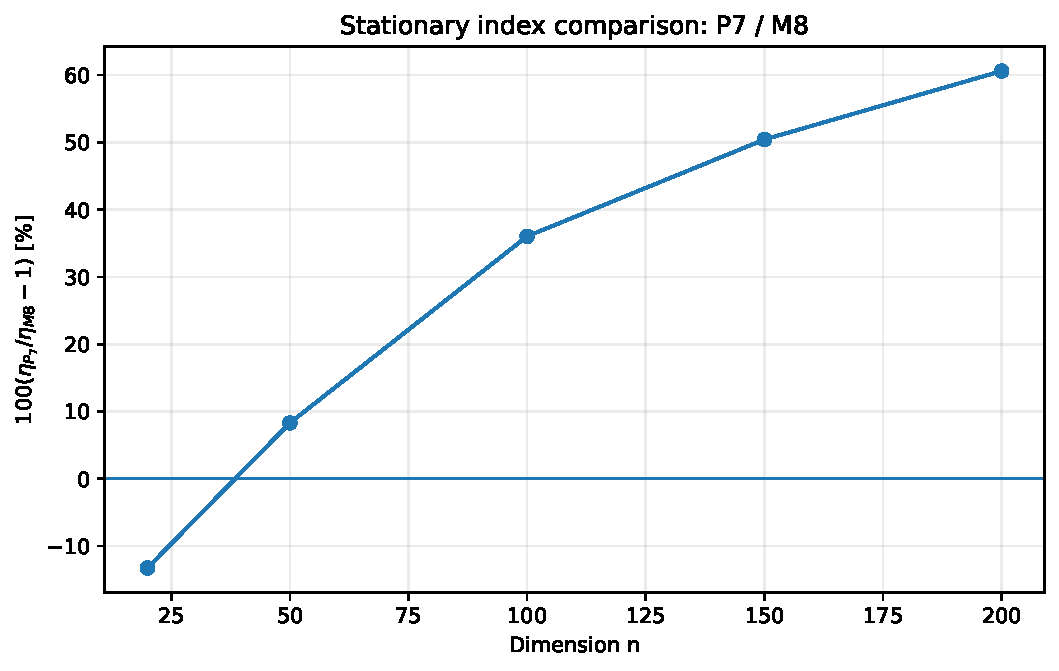
\includegraphics[width=.49\textwidth]{figures/supp_figS1_index.pdf}\hfill
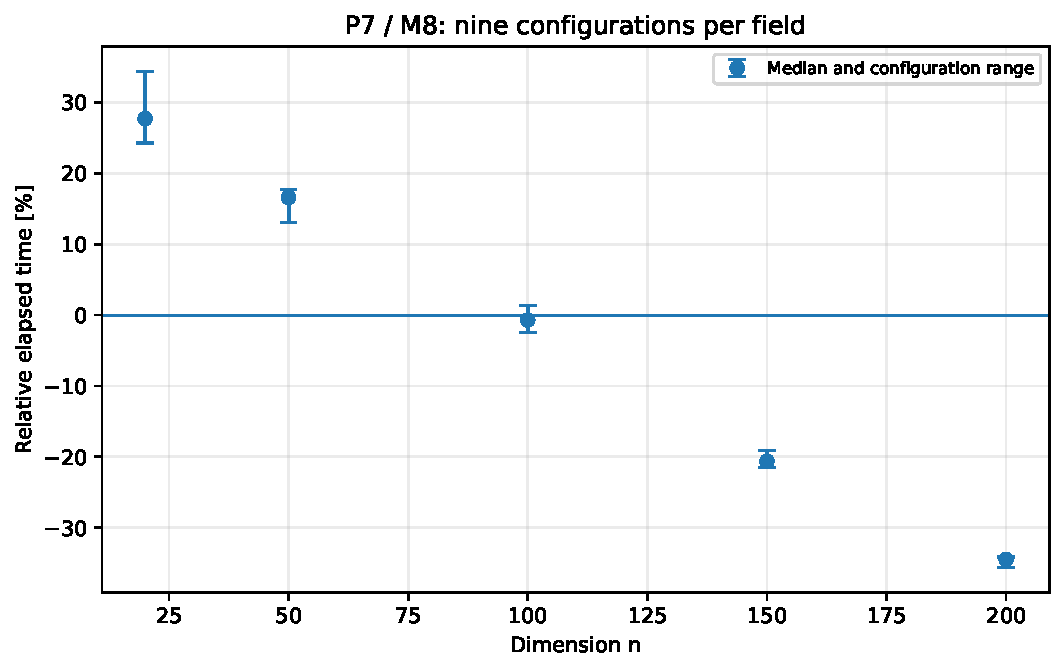
\includegraphics[width=.49\textwidth]{figures/supp_figS1_time.pdf}
\caption{$P_7/M8$: stationary index advantage (left) and median with configuration range of relative elapsed time (right). Positive index differences and negative time differences favor $P_7$. The displayed range is not an IQR or confidence interval.}\label{fig:external-time}
\end{figure}
\begin{figure}[htbp]\centering
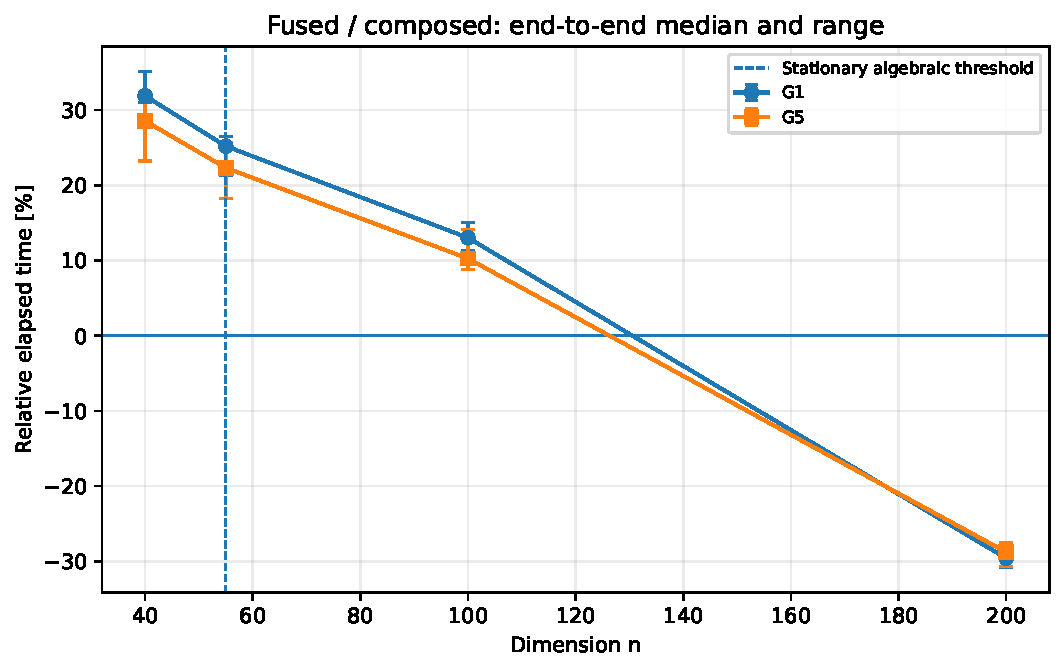
\includegraphics[width=.78\textwidth]{figures/supp_figS2_fusion.pdf}
\caption{End-to-end $\widehat P_2/(P_2\circ P_2)$: median and range of relative elapsed time. The line $n=55$ marks the stationary algebraic threshold, not an estimated temporal crossover. No interpolation establishes universal monotonicity.}\label{fig:fusion-time}
\end{figure}
Figures~\ref{fig:external-time} and~\ref{fig:fusion-time} are additional views of the same archived timing summaries. The efficiency-region figures in the article answer a different question: how the stationary favorable set varies with $(\mu_0,\mu_1)$ and dimension.

\clearpage
\section{Multiprecision comparison of independently selected family optima}\label{sec:mp-data}
All eight groups in the frozen family plan are complete. Table~\ref{tab:mp-coverage} states the coverage. The dataset contains 496 individual timed full solves, or 248 paired repetitions, across 16 method configurations. The four H1 groups share one recorded session; each H5 tolerance has a separate session, for five sessions in total. Within each group, both methods were interleaved in the same session. No pilot sample, partial group or across-session splice is included.

The comparison remains $P_3/S_3$ in $H_1$ ($n=20$) and $P_9/S_{10}$ in $H_5$ ($n=200$), the independent optima of the canonical reference-index model at $\kappa=1$. These are not calibrated multiprecision time optima. The central distance $\delta=0.30$ and all four initially proposed tolerances were retained in this resource-limited tranche. The plan was frozen after feasibility pilots and before repeated timing runs. Pilot outcomes were visible at the design decision; blinded selection is not claimed.

\begin{table}[htbp]\centering\small
\caption{Complete frozen family plan. Every group contains 31 repetitions of each method.}\label{tab:mp-coverage}
\begin{tabular}{cccl}\toprule
Field & Pair & TOL & Status\\\midrule
$H_{1}$ & $P_{3}/S_{3}$ & $10^{-50}$ & Complete\\
$H_{1}$ & $P_{3}/S_{3}$ & $10^{-200}$ & Complete\\
$H_{1}$ & $P_{3}/S_{3}$ & $10^{-800}$ & Complete\\
$H_{1}$ & $P_{3}/S_{3}$ & $10^{-1024}$ & Complete\\
$H_{5}$ & $P_{9}/S_{10}$ & $10^{-50}$ & Complete\\
$H_{5}$ & $P_{9}/S_{10}$ & $10^{-200}$ & Complete\\
$H_{5}$ & $P_{9}/S_{10}$ & $10^{-800}$ & Complete\\
$H_{5}$ & $P_{9}/S_{10}$ & $10^{-1024}$ & Complete\\
\bottomrule\end{tabular}\end{table}
\FloatBarrier
\subsection{Execution identity, arithmetic and measured boundaries}
The source and protocol hashes identify the actual frozen files, not a subsequent public release. The source hash is \texttt{f62dd86b}\allowbreak\texttt{1c521d14}\allowbreak\texttt{e1f6e5bd}\allowbreak\texttt{af913248}\allowbreak\texttt{2767b5be}\allowbreak\texttt{157758c2}\allowbreak\texttt{9b9e2ae7}\allowbreak\texttt{7f3dc66d} and the protocol hash is \texttt{7eddefb2}\allowbreak\texttt{878492a4}\allowbreak\texttt{ed2d4d37}\allowbreak\texttt{db8f6b3d}\allowbreak\texttt{74de79f3}\allowbreak\texttt{42298462}\allowbreak\texttt{b8e5e895}\allowbreak\texttt{0e489def}. The original driver hashes file bytes indexed by platform-native relative paths; the audit reconstructs Windows separators when checking this identity on another platform. Program bytes are unchanged.

All five session records agree on Windows-11-10.0.26200-SP0; AMD64 Family 25 Model 80 Stepping 0, AuthenticAMD; Python 3.13.6; NumPy 2.3.2; mpmath 1.3.0, Python backend; and no gmpy2. The solver is serial, uses mpmath numbers in object arrays and does not call BLAS. A generic partial-pivoting LU is computed in multiprecision and reused by triangular solves; no inverse or special low-rank representation is formed. Six coefficient matrices (A/B/C at dimensions 20 and 200) agree bytewise with the prescribed PCG64 realization.

The float64 coefficient matrices are lifted as exact dyadic data. Decimal analytic constants and $\alpha_j=j/10$ are evaluated at the current precision. One initial vector constructed at 1300 digits is frozen and lifted exactly for the 2600-digit check. This preserves the coefficient realization but does not reproduce float64 evaluation roundoff. Original $x$ coordinates are iterated. Problem generation and constant matrix prescaling are outside the timer.

The settings are 1300 working digits, 2600 verification digits, delayed D initialization, 20 maximum cycles, two warmups and 31 repetitions. Warmups are specified in the frozen plan and driver but not saved as separate timed observations. The timer is \texttt{time.perf\_counter\_ns}, using the recorded monotonic QueryPerformanceCounter clock. It measures the complete solve, including copies, counters, numerical operations and residual tests. Error norms, trace serialization, I/O, precision gates and statistical aggregation are outside that interval. Integer nanosecond readings do not imply nanosecond experimental accuracy.

Every repetition has one measurement of each method in deterministic pseudo-random order. Exact order, durations, status, resources and final error/residual strings are retained under \texttt{data/multiprecision/families/sessions}. Each completed-group marker identifies its session. For H5 the session starts are September 26, 2026, at 04:35, 16:20 and 19:13 UTC for $d=50,200,800$, and September 27 at 12:17 UTC for $d=1024$. The H1 session starts on September 26 at 04:31 UTC. These identify recorded invocations, not independent replications of the hardware experiment.

\subsection{Complete timing and work summaries}
All eight groups, favorable or otherwise, appear below. Times are seconds, unlike the earlier millisecond tables. Reference work uses the unchanged model, not physical scalar-operation weights calibrated for multiprecision.
\begin{table}[htbp]\centering\scriptsize\setlength{\tabcolsep}{3pt}
\caption{All eight family comparisons: $P_3/S_3$ in $H_1$ and $P_9/S_{10}$ in $H_5$. Times are seconds with IQRs in parentheses; $d$ denotes TOL $=10^{-d}$. Negative differences favor $P$. The filter is the two-IQR rule.}\label{tab:mp-summary}
\begin{tabular}{cccrrrrc}\toprule
Field & $d$: TOL $=10^{-d}$ & cycles $P/S$ & $\widetilde t_P$ (IQR) & $\widetilde t_S$ (IQR) & $\Delta t$ [\%] & $\Delta W$ [\%] & filter\\\midrule
$H_{1}$ & 50 & $3/3$ & $0.357824\,(0.138745)$ & $0.355855\,(0.163756)$ & $+0.553$ & $+3.026$ & no\\
$H_{1}$ & 200 & $4/4$ & $0.531415\,(0.058401)$ & $0.502425\,(0.089211)$ & $+5.770$ & $+3.444$ & no\\
$H_{1}$ & 800 & $5/5$ & $0.537007\,(0.009490)$ & $0.528849\,(0.011225)$ & $+1.543$ & $+3.700$ & no\\
$H_{1}$ & 1024 & $5/5$ & $0.530157\,(0.006841)$ & $0.525820\,(0.007198)$ & $+0.825$ & $+3.700$ & no\\
\midrule
$H_{5}$ & 50 & $2/2$ & $134.308598\,(0.385663)$ & $138.014224\,(0.347079)$ & $-2.685$ & $-3.267$ & yes\\
$H_{5}$ & 200 & $2/2$ & $136.036516\,(3.976849)$ & $140.439827\,(4.375426)$ & $-3.135$ & $-3.267$ & no\\
$H_{5}$ & 800 & $3/3$ & $190.385437\,(2.253746)$ & $192.323630\,(1.502451)$ & $-1.008$ & $-3.133$ & no\\
$H_{5}$ & 1024 & $3/3$ & $188.605813\,(0.335320)$ & $191.176665\,(1.062469)$ & $-1.345$ & $-3.133$ & no\\
\bottomrule\end{tabular}\end{table}

\FloatBarrier
The H1 medians favor S3 in all four configurations, by 0.553\% to 5.770\% relative to S3, without crossing the descriptive two-IQR filter. At $10^{-200}$ P3 produces a much smaller error without saving a cycle. The additional predictor solves increase its reference work by 3.026\% to 3.700\%.

In H5, P9 has lower medians at all four tolerances: reductions of 2.685\%, 3.135\%, 1.008\% and 1.345\% in increasing $d$ order. Only the $10^{-50}$ difference passes the two-IQR filter. For $10^{-1024}$, the difference of medians is 2.5708524 s, below the 2.7955777 s threshold. P9 and S10 use two cycles for $d=50,200$ and three for $d=800,1024$; P9 activates inherited memory in one or two cycles, respectively. Its reference-work reduction is 3.267\% for the two-cycle runs and 3.133\% for the three-cycle runs. No family comparison saves an outer cycle. Because correction counts also differ, the H5 outcome supports those optimized pairs in their recorded sessions, not a causal isolation of memory.

\begin{table}[htbp]\centering\scriptsize
\caption{Exact total resources, including the terminal residual evaluation. Here $d$ denotes TOL $=10^{-d}$. Additional matrix--vector products and comparator scalings are zero for these family runs.}\label{tab:mp-resources}
\begin{tabular}{cccrrrrrr}\toprule
Field & $d$ & Method & cycles & active memory & F & J / LU & solves & work\\\midrule
$H_{1}$ & 50 & $P_{3}$ & 3 & 2 & 10 & 3 / 3 & 11 & 27240\\
$H_{1}$ & 50 & $S_{3}$ & 3 & 0 & 10 & 3 / 3 & 9 & 26440\\
$H_{1}$ & 200 & $P_{3}$ & 4 & 3 & 13 & 4 / 4 & 15 & 36040\\
$H_{1}$ & 200 & $S_{3}$ & 4 & 0 & 13 & 4 / 4 & 12 & 34840\\
$H_{1}$ & 800 & $P_{3}$ & 5 & 4 & 16 & 5 / 5 & 19 & 44840\\
$H_{1}$ & 800 & $S_{3}$ & 5 & 0 & 16 & 5 / 5 & 15 & 43240\\
$H_{1}$ & 1024 & $P_{3}$ & 5 & 4 & 16 & 5 / 5 & 19 & 44840\\
$H_{1}$ & 1024 & $S_{3}$ & 5 & 0 & 16 & 5 / 5 & 15 & 43240\\
\midrule
$H_{5}$ & 50 & $P_{9}$ & 2 & 1 & 19 & 2 / 2 & 19 & 8658200\\
$H_{5}$ & 50 & $S_{10}$ & 2 & 0 & 21 & 2 / 2 & 20 & 8950600\\
$H_{5}$ & 200 & $P_{9}$ & 2 & 1 & 19 & 2 / 2 & 19 & 8658200\\
$H_{5}$ & 200 & $S_{10}$ & 2 & 0 & 21 & 2 / 2 & 20 & 8950600\\
$H_{5}$ & 800 & $P_{9}$ & 3 & 2 & 28 & 3 / 3 & 29 & 12944200\\
$H_{5}$ & 800 & $S_{10}$ & 3 & 0 & 31 & 3 / 3 & 30 & 13362800\\
$H_{5}$ & 1024 & $P_{9}$ & 3 & 2 & 28 & 3 / 3 & 29 & 12944200\\
$H_{5}$ & 1024 & $S_{10}$ & 3 & 0 & 31 & 3 / 3 & 30 & 13362800\\
\bottomrule\end{tabular}\end{table}
\FloatBarrier
\subsection{Paired bootstrap and descriptive separation}
For each of 10000 bootstrap resamples, 31 pair indices are drawn with replacement and the same indices are used for both methods. The statistic is the ratio of the resampled medians, not the median of within-pair ratios. The 2.5th and 97.5th percentiles give Table~\ref{tab:mp-bootstrap}; the deterministic seed follows from the frozen driver, plan and group ID.
\begin{table}[htbp]\centering\small
\caption{Ratio of medians and pointwise paired percentile bootstrap intervals (nominal 95\%). No multiplicity or serial-dependence correction is applied.}\label{tab:mp-bootstrap}
\begin{tabular}{ccrrrc}\toprule
Field & $d$ & ratio P/S & lower & upper & two-IQR filter\\\midrule
$H_{1}$ & 50 & 1.005532 & 0.889939 & 1.075961 & no\\
$H_{1}$ & 200 & 1.057699 & 0.976482 & 1.088468 & no\\
$H_{1}$ & 800 & 1.015425 & 1.009291 & 1.020359 & no\\
$H_{1}$ & 1024 & 1.008248 & 1.003821 & 1.014380 & no\\
\midrule
$H_{5}$ & 50 & 0.973150 & 0.972079 & 0.974394 & yes\\
$H_{5}$ & 200 & 0.968646 & 0.957478 & 0.977008 & no\\
$H_{5}$ & 800 & 0.989922 & 0.987533 & 0.994525 & no\\
$H_{5}$ & 1024 & 0.986552 & 0.984817 & 0.987467 & no\\
\bottomrule\end{tabular}\end{table}
\FloatBarrier
The criteria are not interchangeable. The H1 intervals at $10^{-800}$ and $10^{-1024}$ lie above one, although the two-IQR rule is not met; at $10^{-50}$ and $10^{-200}$ they include one. All four H5 intervals lie below one, but only its $10^{-50}$ group passes the two-IQR filter. Failure to pass the latter is not evidence of equal times. These summaries are conditional on the recorded sessions and sampling design; they do not establish universal superiority or a quantitative overhead model. No historical IQR-only table is bootstrapped.

\subsection{Precision checks, termination and saved trajectories}
Each method was checked before its repeated timings at 1300 and 2600 digits, using the same frozen start. The final low-precision iterate was also reevaluated at 2600 digits. All sixteen checks pass and cycle counts agree. The audit recalculates error norms and COC from the saved exact dyadics and independently evaluates the final residuals by row-wise sums of the stated field formula. These are numerical checks, not interval certification.

The comparison uses the floor and criterion
\[
 f=10^{-1300+40}(1+\|\alpha\|_2),\qquad
 \frac{\|x_k^{(1300)}-x_k^{(2600)}\|_2}{\max\{\|x_k^{(2600)}-\alpha\|_2,f\}}<10^{-10}.
\]
A high-precision error below $f$ triggers a floor-censored flag; passing the test then is not a relative-accuracy certificate. Separately, the reevaluated low-precision final iterate must meet the requested residual tolerance.
\begin{table}[htbp]\centering\scriptsize
\caption{Final 1300-digit iterate reevaluated at 2600 digits. The floor column denotes a censored precision comparison, not failure to meet the tolerance.}\label{tab:mp-precision}
\begin{tabular}{cccrrc}\toprule
Field & $d$ & Method & checked residual & checked error & final floor\\\midrule
$H_{1}$ & 50 & $P_{3}$ & $1.375\times10^{-153}$ & $3.396\times10^{-154}$ & no\\
$H_{1}$ & 50 & $S_{3}$ & $1.785\times10^{-120}$ & $4.526\times10^{-121}$ & no\\
$H_{1}$ & 200 & $P_{3}$ & $7.705\times10^{-705}$ & $1.956\times10^{-705}$ & no\\
$H_{1}$ & 200 & $S_{3}$ & $2.284\times10^{-485}$ & $5.385\times10^{-486}$ & no\\
$H_{1}$ & 800 & $P_{3}$ & $6.733\times10^{-1301}$ & $1.697\times10^{-1301}$ & yes\\
$H_{1}$ & 800 & $S_{3}$ & $6.733\times10^{-1301}$ & $1.697\times10^{-1301}$ & yes\\
$H_{1}$ & 1024 & $P_{3}$ & $6.733\times10^{-1301}$ & $1.697\times10^{-1301}$ & yes\\
$H_{1}$ & 1024 & $S_{3}$ & $6.733\times10^{-1301}$ & $1.697\times10^{-1301}$ & yes\\
\midrule
$H_{5}$ & 50 & $P_{9}$ & $2.637\times10^{-286}$ & $6.679\times10^{-287}$ & no\\
$H_{5}$ & 50 & $S_{10}$ & $7.598\times10^{-321}$ & $1.941\times10^{-321}$ & no\\
$H_{5}$ & 200 & $P_{9}$ & $2.637\times10^{-286}$ & $6.679\times10^{-287}$ & no\\
$H_{5}$ & 200 & $S_{10}$ & $7.598\times10^{-321}$ & $1.941\times10^{-321}$ & no\\
$H_{5}$ & 800 & $P_{9}$ & $2.536\times10^{-1299}$ & $6.371\times10^{-1300}$ & yes\\
$H_{5}$ & 800 & $S_{10}$ & $2.536\times10^{-1299}$ & $6.371\times10^{-1300}$ & yes\\
$H_{5}$ & 1024 & $P_{9}$ & $2.536\times10^{-1299}$ & $6.371\times10^{-1300}$ & yes\\
$H_{5}$ & 1024 & $S_{10}$ & $2.536\times10^{-1299}$ & $6.371\times10^{-1300}$ & yes\\
\bottomrule\end{tabular}\end{table}
\FloatBarrier
For H1 at $10^{-800}$ and $10^{-1024}$, the final computed error and residual are zero, but the saved iterate has a reevaluated residual of $6.7330\times10^{-1301}$. For H5 at both stringent tolerances, the reevaluated residual is $2.5362\times10^{-1299}$, again below the requested tolerance despite computed zero finals. No COC is formed with these zeros. In H5, the only nonzero-error COC uses the initial transient; its third-cycle final is zero at both working precisions. Thus this H5 campaign supplies no wholly post-startup COC. The established order-verification study remains separate.

Eight nominal paired configurations correspond to five paired exact paths in two fields. Equality was checked directly on every stored dyadic iterate, at both precisions, within each repeated-path pair: H1 at $d=800/1024$, H5 at $d=50/200$, and H5 at $d=800/1024$. These duplicated paths are not additional nonlinear problems. In particular, the H5 differences in median and IQR between $d=50$ and $d=200$, or between $d=800$ and $d=1024$, are not attributed to an algorithmic path change; they were timed in different sessions. All measured outcomes are retained.

Table~\ref{tab:mp-traces} displays the longest saved path in each field at both precisions. Every per-group trace remains in \texttt{data/multiprecision/families/audit/stored\_trace\_summary.csv}, and the exact vectors are in the compressed gate files. A dash denotes an unavailable COC, not zero. The shorter-tolerance paths are prefixes, checked against these saved vectors.
\begingroup\scriptsize\setlength{\tabcolsep}{3.5pt}
\begin{longtable}{cccrrrrc}
\caption{Saved trajectory diagnostics at $10^{-1024}$ for both fields. Shorter-tolerance runs follow prefixes of these paths. ``Tail'' requires a defined COC wholly after the initial block; a zero final is not used for COC.}\label{tab:mp-traces}\\
\toprule Field & Method & digits & $k$ & error & residual & COC & tail\\\midrule\endfirsthead
\multicolumn{8}{c}{Table \thetable\ continued}\\\toprule Field & Method & digits & $k$ & error & residual & COC & tail\\\midrule\endhead
\bottomrule\endfoot
$H_{1}$ & $P_{3}$ & 1300 & 0 & $3.000\times10^{-1}$ & $1.233\times10^{0}$ & -- & no\\
$H_{1}$ & $P_{3}$ & 1300 & 1 & $5.489\times10^{-7}$ & $2.286\times10^{-6}$ & -- & no\\
$H_{1}$ & $P_{3}$ & 1300 & 2 & $2.434\times10^{-33}$ & $9.356\times10^{-33}$ & 4.593070 & no\\
$H_{1}$ & $P_{3}$ & 1300 & 3 & $3.396\times10^{-154}$ & $1.375\times10^{-153}$ & 4.585969 & yes\\
$H_{1}$ & $P_{3}$ & 1300 & 4 & $1.956\times10^{-705}$ & $7.705\times10^{-705}$ & 4.561155 & yes\\
$H_{1}$ & $P_{3}$ & 1300 & 5 & $0$ & $0$ & -- & no\\
$H_{1}$ & $P_{3}$ & 2600 & 0 & $3.000\times10^{-1}$ & $1.233\times10^{0}$ & -- & no\\
$H_{1}$ & $P_{3}$ & 2600 & 1 & $5.489\times10^{-7}$ & $2.286\times10^{-6}$ & -- & no\\
$H_{1}$ & $P_{3}$ & 2600 & 2 & $2.434\times10^{-33}$ & $9.356\times10^{-33}$ & 4.593070 & no\\
$H_{1}$ & $P_{3}$ & 2600 & 3 & $3.396\times10^{-154}$ & $1.375\times10^{-153}$ & 4.585969 & yes\\
$H_{1}$ & $P_{3}$ & 2600 & 4 & $1.956\times10^{-705}$ & $7.705\times10^{-705}$ & 4.561155 & yes\\
$H_{1}$ & $P_{3}$ & 2600 & 5 & $0$ & $0$ & -- & no\\
$H_{1}$ & $S_{3}$ & 1300 & 0 & $3.000\times10^{-1}$ & $1.233\times10^{0}$ & -- & no\\
$H_{1}$ & $S_{3}$ & 1300 & 1 & $5.489\times10^{-7}$ & $2.286\times10^{-6}$ & -- & no\\
$H_{1}$ & $S_{3}$ & 1300 & 2 & $8.761\times10^{-30}$ & $3.620\times10^{-29}$ & 3.973242 & no\\
$H_{1}$ & $S_{3}$ & 1300 & 3 & $4.526\times10^{-121}$ & $1.785\times10^{-120}$ & 4.004346 & yes\\
$H_{1}$ & $S_{3}$ & 1300 & 4 & $5.385\times10^{-486}$ & $2.284\times10^{-485}$ & 3.997560 & yes\\
$H_{1}$ & $S_{3}$ & 1300 & 5 & $0$ & $0$ & -- & no\\
$H_{1}$ & $S_{3}$ & 2600 & 0 & $3.000\times10^{-1}$ & $1.233\times10^{0}$ & -- & no\\
$H_{1}$ & $S_{3}$ & 2600 & 1 & $5.489\times10^{-7}$ & $2.286\times10^{-6}$ & -- & no\\
$H_{1}$ & $S_{3}$ & 2600 & 2 & $8.761\times10^{-30}$ & $3.620\times10^{-29}$ & 3.973242 & no\\
$H_{1}$ & $S_{3}$ & 2600 & 3 & $4.526\times10^{-121}$ & $1.785\times10^{-120}$ & 4.004346 & yes\\
$H_{1}$ & $S_{3}$ & 2600 & 4 & $5.385\times10^{-486}$ & $2.284\times10^{-485}$ & 3.997560 & yes\\
$H_{1}$ & $S_{3}$ & 2600 & 5 & $1.231\times10^{-1945}$ & $5.098\times10^{-1945}$ & 3.999843 & yes\\
$H_{5}$ & $P_{9}$ & 1300 & 0 & $3.000\times10^{-1}$ & $1.223\times10^{0}$ & -- & no\\
$H_{5}$ & $P_{9}$ & 1300 & 1 & $2.752\times10^{-25}$ & $1.076\times10^{-24}$ & -- & no\\
$H_{5}$ & $P_{9}$ & 1300 & 2 & $6.679\times10^{-287}$ & $2.637\times10^{-286}$ & 10.883595 & no\\
$H_{5}$ & $P_{9}$ & 1300 & 3 & $0$ & $0$ & -- & no\\
$H_{5}$ & $P_{9}$ & 2600 & 0 & $3.000\times10^{-1}$ & $1.223\times10^{0}$ & -- & no\\
$H_{5}$ & $P_{9}$ & 2600 & 1 & $2.752\times10^{-25}$ & $1.076\times10^{-24}$ & -- & no\\
$H_{5}$ & $P_{9}$ & 2600 & 2 & $6.679\times10^{-287}$ & $2.637\times10^{-286}$ & 10.883595 & no\\
$H_{5}$ & $P_{9}$ & 2600 & 3 & $0$ & $0$ & -- & no\\
$H_{5}$ & $S_{10}$ & 1300 & 0 & $3.000\times10^{-1}$ & $1.223\times10^{0}$ & -- & no\\
$H_{5}$ & $S_{10}$ & 1300 & 1 & $6.208\times10^{-28}$ & $2.414\times10^{-27}$ & -- & no\\
$H_{5}$ & $S_{10}$ & 1300 & 2 & $1.941\times10^{-321}$ & $7.598\times10^{-321}$ & 10.999222 & no\\
$H_{5}$ & $S_{10}$ & 1300 & 3 & $0$ & $0$ & -- & no\\
$H_{5}$ & $S_{10}$ & 2600 & 0 & $3.000\times10^{-1}$ & $1.223\times10^{0}$ & -- & no\\
$H_{5}$ & $S_{10}$ & 2600 & 1 & $6.208\times10^{-28}$ & $2.414\times10^{-27}$ & -- & no\\
$H_{5}$ & $S_{10}$ & 2600 & 2 & $1.941\times10^{-321}$ & $7.598\times10^{-321}$ & 10.999222 & no\\
$H_{5}$ & $S_{10}$ & 2600 & 3 & $0$ & $0$ & -- & no\\
\end{longtable}\endgroup

\subsection{Completed scope and provenance}
All eight planned family groups have completion markers, with 496 raw timing observations and sixteen precision gates. No value is borrowed from a pilot or inferred from cycle counts. The multiprecision timing evidence concerns only the stated optimum-family comparisons at $\delta=0.30$. This section concerns only the family comparison. External multiprecision measurements are reported separately below; the preceding fused-$q$ timing tables still concern float64 measurements.

Original files are preserved bytewise under \texttt{data/multiprecision/families}; reconstructed summaries and the numerical audit are under \texttt{data/multiprecision/families/audit}; the exact solver snapshot is under \texttt{experiments/multiprecision/families}. The code, frozen protocol and previously supplied five groups remain unchanged. The multiprecision data and expanded supplement are distributed with the repository and are not claimed to belong to Zenodo v1.0.0.


\clearpage
\section{External multiprecision comparisons with platform-resolved allocation}\label{sec:external-mp}
The external campaign contains all 16 planned groups: $P_5/M6$ and $P_7/M8$, $H_1$ ($n=20$) and $H_5$ ($n=200$), $\delta=0.30$, and residual tolerances $10^{-d}$ for $d=50,200,800,1024$. It is separate from the family-optimum campaign and from the earlier float64 external timings. All methods use the stated field, exact-dyadic coefficient lift, original $x$ coordinates, 1300 working digits, 2600 verification digits, partial-pivoting LU reuse and delayed initialization D for $P_N$.

\subsection{Allocation, platform provenance and measurement boundaries}
Each group starts with two warmups and 15 paired repetitions. The predeclared rule keeps 15 only when the paired-bootstrap percentile interval excludes one, the two-IQR filter is met, and both favor the same method. Otherwise 16 additional pairs are collected, preceded by new gates and warmups. The initial fixed-size data and decisions are unchanged byte for byte. Eight groups were extended and eight stopped at 15: 736 timed solves, 368 pairs, 32 method configurations and 48 stored precision gates. Warmups are documented by the frozen code and plan, not separately saved as timing observations.

Twelve groups (all eight $P_5/M6$ groups and the four $P_7/M8$ groups in $H_1$) use the AMD environment. The four $P_7/M8$ groups in $H_5$ use Intel, each with 15 pairs and no extension. All eight extensions in the current aggregate use AMD, matching their initial phases. There are 16 initial sessions and eight extension sessions; 616 current measurements are AMD and 120 are Intel. No current group pools hardware platforms. Matching platform metadata does not make separate sessions identically distributed or independent.

\begin{table}[htbp]\centering\small
\caption{Recorded platforms of the external campaign. ``AMD64'' in a machine-architecture field is not used to identify the processor vendor.}\label{tab:ext-platforms}
\begin{tabularx}{\textwidth}{lXX}\toprule
 & AMD & Intel\\\midrule
Processor & AMD64 Family 25 Model 80 Stepping 0, AuthenticAMD & Intel64 Family 6 Model 151 Stepping 2, GenuineIntel\\
Python & 3.13.6 & 3.13.5\\
Logical CPUs reported & 16 & 20\\
OS & Windows-11-10.0.26200-SP0 & Windows-11-10.0.26200-SP0\\
NumPy / mpmath & 2.3.2 / 1.3.0 & 2.3.2 / 1.3.0\\
Arithmetic & Python backend; no gmpy2 & Python backend; no gmpy2\\
Current groups & 12 & 4\\\bottomrule
\end{tabularx}\end{table}
\FloatBarrier

The solver is serial and does not use BLAS. The monotonic \texttt{perf\_counter\_ns} timer wraps the full solve, including copies, counters, scalar/matrix operations and terminal residual tests; it excludes problem setup, error-norm reporting, trace serialization, I/O, gates, warmups and aggregation. Every pair contains one run of each method in a reproducible randomized order. The trial cap is 20 cycles. Full session identifiers and recorded settings are in \texttt{data/multiprecision/external/audit/platform\_sessions.csv}.

The repeated protocol was frozen on September 27, 2026, before initial timings; allocation decisions were recorded on September 29 after those 16 groups. Eight earlier follow-ups used Intel. They are preserved separately; replacement AMD follow-ups ran on September 30--October 1 using the same eight decisions and no newly selected tolerances. Earlier follow-up outcomes were already visible, so blinded replacement is not claimed. The four unextended $P_7/M8$ groups in $H_5$ remain Intel; they must not be relabeled as AMD or interpreted as an AMD dimension sweep.

\subsection{Final descriptive timing summaries}
\begin{table}[htbp]
\centering\scriptsize
\setlength{\tabcolsep}{3pt}
\caption{External $P_5/M6$ timings. Seconds; IQR in parentheses. Platforms are identified per row. Negative changes favor $P_5$. The adaptive aggregate combines only the same reported platform, but extended groups span two sessions.}\label{tab:ext-external6}
\begin{tabular}{cccccrrrc}\toprule
Field & platform & $d$ & pairs & cycles & $P_5$ median (IQR) & $M6$ median (IQR) & change [\%] & filter\\\midrule
$H_1$ & AMD & 50 & 31 & $2/2$ & $0.312290\,(0.007706)$ & $0.302739\,(0.005472)$ & +3.155 & no\\
$H_1$ & AMD & 200 & 31 & $3/3$ & $0.462004\,(0.008549)$ & $0.447156\,(0.008603)$ & +3.321 & no\\
$H_1$ & AMD & 800 & 31 & $4/4$ & $0.553661\,(0.008682)$ & $0.572815\,(0.008094)$ & -3.344 & no\\
$H_1$ & AMD & 1024 & 31 & $4/4$ & $0.556572\,(0.010900)$ & $0.571583\,(0.012388)$ & -2.626 & no\\
$H_5$ & AMD & 50 & 15 & $2/2$ & $114.474034\,(0.426745)$ & $112.138516\,(0.160686)$ & +2.083 & yes\\
$H_5$ & AMD & 200 & 31 & $3/3$ & $173.749752\,(2.623016)$ & $168.895049\,(2.464180)$ & +2.874 & no\\
$H_5$ & AMD & 800 & 31 & $4/4$ & $228.295552\,(9.249476)$ & $227.487334\,(8.264110)$ & +0.355 & no\\
$H_5$ & AMD & 1024 & 31 & $4/4$ & $222.429909\,(2.535950)$ & $221.004646\,(2.961342)$ & +0.645 & no\\
\bottomrule\end{tabular}
\end{table}
\FloatBarrier

\begin{table}[htbp]
\centering\scriptsize
\setlength{\tabcolsep}{3pt}
\caption{External $P_7/M8$ timings. Seconds; IQR in parentheses. Platforms are identified per row. Negative changes favor $P_7$. The adaptive aggregate combines only the same reported platform, but extended groups span two sessions.}\label{tab:ext-external8}
\begin{tabular}{cccccrrrc}\toprule
Field & platform & $d$ & pairs & cycles & $P_7$ median (IQR) & $M8$ median (IQR) & change [\%] & filter\\\midrule
$H_1$ & AMD & 50 & 31 & $2/2$ & $0.385014\,(0.009912)$ & $0.361616\,(0.008927)$ & +6.470 & no\\
$H_1$ & AMD & 200 & 15 & $3/3$ & $0.585748\,(0.007271)$ & $0.537445\,(0.009296)$ & +8.988 & yes\\
$H_1$ & AMD & 800 & 15 & $3/3$ & $0.579601\,(0.005976)$ & $0.536758\,(0.007237)$ & +7.982 & yes\\
$H_1$ & AMD & 1024 & 15 & $3/4$ & $0.580049\,(0.003926)$ & $0.680062\,(0.003980)$ & -14.706 & yes\\
$H_5$ & Intel & 50 & 15 & $2/2$ & $100.705191\,(0.402399)$ & $161.158137\,(0.502481)$ & -37.512 & yes\\
$H_5$ & Intel & 200 & 15 & $3/3$ & $148.041299\,(0.340894)$ & $241.791999\,(0.263207)$ & -38.773 & yes\\
$H_5$ & Intel & 800 & 15 & $3/3$ & $147.898461\,(0.562725)$ & $241.762238\,(0.628141)$ & -38.825 & yes\\
$H_5$ & Intel & 1024 & 15 & $3/3$ & $148.493841\,(0.610147)$ & $241.748945\,(0.690050)$ & -38.575 & yes\\
\bottomrule\end{tabular}
\end{table}
\FloatBarrier

For $P_5/M6$, both methods require 2, 3, 4 and 4 cycles as $d$ increases, in both fields. In $H_1$, $P_5$ has higher medians at $d=50,200$ and lower medians at $800,1024$, with no two-IQR separation. In $H_5$ its medians are always higher; only $d=50$ passes the filter, favoring $M6$. Reference work is higher for $P_5$ in all eight groups. Neither this model mismatch nor an unpassed filter is used to assert equal execution times.

For $P_7/M8$ in $H_1$, the first three medians favor $M8$; the $d=200,800$ differences pass the filter. At $d=1024$, $P_7$ takes three cycles against four, lowers the median by 14.706\% and lowers reference work by 10.252\%. In $H_5$ (Intel), both methods take 2, 3, 3 and 3 cycles; $P_7$ lowers the four medians by 37.512--38.825\%, and all four differences pass the filter. Its reference-work reduction is about 34.94\%. The comparison is within the recorded Intel platform; comparing these reductions to $H_1$ does not isolate dimension from hardware.

The predictor is active in every $P_5/P_7$ group. A saved cycle occurs only for $P_7/M8$ in $H_1$ at $d=1024$. The experiment compares complete algorithms, not an intervention that isolates the predictor while fixing all other evaluation and factorization counts.

\subsection{Session phases and bootstrap limitations}
\begin{table}[htbp]
\centering\scriptsize
\setlength{\tabcolsep}{3pt}
\caption{Extended groups: absolute median wall times by AMD session phase (seconds). Each initial phase has 15 pairs and each follow-up has 16. The ratios have the same direction in the two phases for all eight groups; their magnitudes and dispersions need not agree.}\label{tab:ext-phases}
\begin{tabular}{lcrrrrrrr}\toprule
Pair & field & $d$ & initial A & initial B & follow-up A & follow-up B & initial ratio & follow-up ratio\\\midrule
$P_{5}/M6$ & H1 & 50 & 0.307206 & 0.299413 & 0.313455 & 0.304820 & 1.026028 & 1.028329\\
$P_{5}/M6$ & H1 & 200 & 0.459218 & 0.444463 & 0.465256 & 0.450878 & 1.033197 & 1.031889\\
$P_{5}/M6$ & H1 & 800 & 0.552856 & 0.573300 & 0.554224 & 0.570312 & 0.964340 & 0.971790\\
$P_{5}/M6$ & H1 & 1024 & 0.552425 & 0.568990 & 0.560870 & 0.577600 & 0.970887 & 0.971035\\
$P_{7}/M8$ & H1 & 50 & 0.383449 & 0.361157 & 0.386268 & 0.364850 & 1.061722 & 1.058703\\
$P_{5}/M6$ & H5 & 200 & 176.126698 & 171.044699 & 173.685327 & 168.858873 & 1.029712 & 1.028583\\
$P_{5}/M6$ & H5 & 800 & 229.406337 & 229.357006 & 222.010974 & 221.114813 & 1.000215 & 1.004053\\
$P_{5}/M6$ & H5 & 1024 & 224.263011 & 223.337591 & 221.592648 & 220.372374 & 1.004144 & 1.005537\\
\bottomrule\end{tabular}
\end{table}
\FloatBarrier

The current AMD follow-ups retain the direction of the initial ratio in all eight extended groups. Their medians and IQRs need not be stationary across dates. The 31-pair aggregate is a descriptive mixture of two same-platform session samples with fixed sizes 15 and 16, not a single uninterrupted 31-pair experiment. All eight extended aggregates fail the two-IQR filter; additional observations are not guaranteed to produce separation.

\begin{table}[htbp]
\centering\scriptsize
\setlength{\tabcolsep}{3pt}
\caption{Paired-bootstrap percentile diagnostics (2.5th and 97.5th percentiles, 10000 resamples): initial fixed-size sample, final adaptive aggregate, and phase-stratified sensitivity. The latter retains 15/16 pairs per phase. None is claimed to have 95\% coverage after adaptive allocation; a dash means no extension.}\label{tab:ext-bootstrap}
\begin{tabular}{lccccll}\toprule
Pair & field & $d$ & final pairs & initial interval & final interval & stratified interval\\\midrule
$P_{5}/M6$ & H1 & 50 & 31 & $[1.022911,1.042705]$ & $[1.016530,1.036571]$ & $[1.019026,1.036571]$\\
$P_{5}/M6$ & H1 & 200 & 31 & $[1.020311,1.039386]$ & $[1.023216,1.040560]$ & $[1.023216,1.040057]$\\
$P_{5}/M6$ & H1 & 800 & 31 & $[0.956404,0.973812]$ & $[0.958348,0.974457]$ & $[0.958540,0.974457]$\\
$P_{5}/M6$ & H1 & 1024 & 31 & $[0.963829,0.976647]$ & $[0.965758,0.980707]$ & $[0.966110,0.980707]$\\
$P_{7}/M8$ & H1 & 50 & 31 & $[1.053063,1.074850]$ & $[1.051398,1.073916]$ & $[1.051423,1.073916]$\\
$P_{7}/M8$ & H1 & 200 & 15 & $[1.078388,1.100528]$ & $[1.078388,1.100528]$ & -\\
$P_{7}/M8$ & H1 & 800 & 15 & $[1.074540,1.089658]$ & $[1.074540,1.089391]$ & -\\
$P_{7}/M8$ & H1 & 1024 & 15 & $[0.848738,0.857983]$ & $[0.848738,0.857983]$ & -\\
$P_{5}/M6$ & H5 & 50 & 15 & $[1.019644,1.022927]$ & $[1.019727,1.023259]$ & -\\
$P_{5}/M6$ & H5 & 200 & 31 & $[1.027951,1.040488]$ & $[1.026264,1.032821]$ & $[1.026264,1.031870]$\\
$P_{5}/M6$ & H5 & 800 & 31 & $[0.990781,1.011756]$ & $[0.998501,1.023605]$ & $[0.998904,1.011997]$\\
$P_{5}/M6$ & H5 & 1024 & 31 & $[1.000931,1.006869]$ & $[1.001457,1.007839]$ & $[1.003710,1.007878]$\\
$P_{7}/M8$ & H5 & 50 & 15 & $[0.623243,0.626631]$ & $[0.623243,0.626631]$ & -\\
$P_{7}/M8$ & H5 & 200 & 15 & $[0.611004,0.612671]$ & $[0.611004,0.612671]$ & -\\
$P_{7}/M8$ & H5 & 800 & 15 & $[0.610620,0.613952]$ & $[0.610635,0.613923]$ & -\\
$P_{7}/M8$ & H5 & 1024 & 15 & $[0.612782,0.615891]$ & $[0.613007,0.615891]$ & -\\
\bottomrule\end{tabular}
\end{table}
\FloatBarrier

The archived runner generates 10000 paired bootstrap resamples and reports the ratio of resampled medians, rather than the median of pairwise ratios. Its exact seeded percentiles are reproduced. The follow-up decision is data-dependent, so predeclaring the decision rule does not by itself establish 95\% coverage for the final percentile intervals. The initial 15-pair sample is displayed for all groups, not only for early-stopped winners. Final intervals are descriptive and are not adjusted for selection, serial dependence or multiple comparisons.

An additional sensitivity diagnostic resamples within the initial and follow-up phases, keeping their respective sizes 15 and 16. Its interval position relative to one agrees with the archived pooled diagnostic in all eight extended groups. This check addresses the fixed phase composition, not adaptive stopping or all dependence. For $P_5/M6$ in $H_5$ at $d=800$ the final intervals contain one; an unpassed two-IQR filter is not generally equivalent to such inclusion. No numerical significance level is claimed for the two-IQR rule.

\clearpage\subsection{Exact resources and numerical validation}
\begin{table}[htbp]
\centering\scriptsize
\setlength{\tabcolsep}{3pt}
\caption{Total resources including the terminal residual. ``Active'' counts outer cycles using an inherited predictor; ``solves/MV'' separates triangular solves from additional matrix--vector products. Reference work uses the canonical weights, not calibrated multiprecision instruction times.}\label{tab:ext-res-external6}
\begin{tabular}{cccrrrrrrr}\toprule
Field & $d$ & method & cycles & active & F & J/LU & solves/MV & scales & work\\\midrule
H1 & 50 & $P_{5}$ & 2 & 1 & 11 & 2/2 & 11/0 & 0 & 25000\\
H1 & 50 & $M6$ & 2 & 0 & 7 & 4/2 & 10/4 & 80 & 22960\\
H1 & 200 & $P_{5}$ & 3 & 2 & 16 & 3/3 & 17/0 & 0 & 37080\\
H1 & 200 & $M6$ & 3 & 0 & 10 & 6/3 & 15/6 & 120 & 33820\\
H1 & 800 & $P_{5}$ & 4 & 3 & 21 & 4/4 & 23/0 & 0 & 49160\\
H1 & 800 & $M6$ & 4 & 0 & 13 & 8/4 & 20/8 & 160 & 44680\\
H1 & 1024 & $P_{5}$ & 4 & 3 & 21 & 4/4 & 23/0 & 0 & 49160\\
H1 & 1024 & $M6$ & 4 & 0 & 13 & 8/4 & 20/8 & 160 & 44680\\
H5 & 50 & $P_{5}$ & 2 & 1 & 11 & 2/2 & 11/0 & 0 & 7328600\\
H5 & 50 & $M6$ & 2 & 0 & 7 & 4/2 & 10/4 & 800 & 7111800\\
H5 & 200 & $P_{5}$ & 3 & 2 & 16 & 3/3 & 17/0 & 0 & 10949800\\
H5 & 200 & $M6$ & 3 & 0 & 10 & 6/3 & 15/6 & 1200 & 10604600\\
H5 & 800 & $P_{5}$ & 4 & 3 & 21 & 4/4 & 23/0 & 0 & 14571000\\
H5 & 800 & $M6$ & 4 & 0 & 13 & 8/4 & 20/8 & 1600 & 14097400\\
H5 & 1024 & $P_{5}$ & 4 & 3 & 21 & 4/4 & 23/0 & 0 & 14571000\\
H5 & 1024 & $M6$ & 4 & 0 & 13 & 8/4 & 20/8 & 1600 & 14097400\\
\bottomrule\end{tabular}
\end{table}
\FloatBarrier

\begin{table}[htbp]
\centering\scriptsize
\setlength{\tabcolsep}{3pt}
\caption{Total resources including the terminal residual. ``Active counts outer cycles using an inherited predictor; ``solves/MV separates triangular solves from additional matrix--vector products. Reference work uses the canonical weights, not calibrated multiprecision instruction times.}\label{tab:ext-res-external8}
\begin{tabular}{cccrrrrrrr}\toprule
Field & $d$ & method & cycles & active & F & J/LU & solves/MV & scales & work\\\midrule
H1 & 50 & $P_{7}$ & 2 & 1 & 15 & 2/2 & 15/0 & 0 & 31560\\
H1 & 50 & $M8$ & 2 & 0 & 7 & 4/4 & 8/0 & 960 & 26760\\
H1 & 200 & $P_{7}$ & 3 & 2 & 22 & 3/3 & 23/0 & 0 & 46920\\
H1 & 200 & $M8$ & 3 & 0 & 10 & 6/6 & 12/0 & 1440 & 39520\\
H1 & 800 & $P_{7}$ & 3 & 2 & 22 & 3/3 & 23/0 & 0 & 46920\\
H1 & 800 & $M8$ & 3 & 0 & 10 & 6/6 & 12/0 & 1440 & 39520\\
H1 & 1024 & $P_{7}$ & 3 & 2 & 22 & 3/3 & 23/0 & 0 & 46920\\
H1 & 1024 & $M8$ & 4 & 0 & 13 & 8/8 & 16/0 & 1920 & 52280\\
H5 & 50 & $P_{7}$ & 2 & 1 & 15 & 2/2 & 15/0 & 0 & 7993400\\
H5 & 50 & $M8$ & 2 & 0 & 7 & 4/4 & 8/0 & 81600 & 12285800\\
H5 & 200 & $P_{7}$ & 3 & 2 & 22 & 3/3 & 23/0 & 0 & 11947000\\
H5 & 200 & $M8$ & 3 & 0 & 10 & 6/6 & 12/0 & 122400 & 18365600\\
H5 & 800 & $P_{7}$ & 3 & 2 & 22 & 3/3 & 23/0 & 0 & 11947000\\
H5 & 800 & $M8$ & 3 & 0 & 10 & 6/6 & 12/0 & 122400 & 18365600\\
H5 & 1024 & $P_{7}$ & 3 & 2 & 22 & 3/3 & 23/0 & 0 & 11947000\\
H5 & 1024 & $M8$ & 3 & 0 & 10 & 6/6 & 12/0 & 122400 & 18365600\\
\bottomrule\end{tabular}
\end{table}
\FloatBarrier

\begin{table}[htbp]
\centering\scriptsize
\setlength{\tabcolsep}{3pt}
\caption{Final 1300-digit iterate reevaluated independently at 2600 digits. The floor flag concerns relative-precision censoring, not failure of the residual stop. Extension trajectories equal the corresponding initial trajectories exactly at both precisions; their repeated checks are preserved in the data.}\label{tab:ext-precision-external6}
\begin{tabular}{cccrrrc}\toprule
Field & $d$ & method & cycles 1300/2600 & checked residual & checked error & floor\\\midrule
H1 & 50 & $P_{5}$ & 2/2 & $1.0118\times10^{-72}$ & $2.5335\times10^{-73}$ & no\\
H1 & 50 & $M6$ & 2/2 & $4.1728\times10^{-64}$ & $9.9401\times10^{-65}$ & no\\
H1 & 200 & $P_{5}$ & 3/3 & $4.7011\times10^{-493}$ & $1.2045\times10^{-493}$ & no\\
H1 & 200 & $M6$ & 3/3 & $2.9827\times10^{-390}$ & $7.2474\times10^{-391}$ & no\\
H1 & 800 & $P_{5}$ & 4/4 & $6.7330\times10^{-1301}$ & $1.6970\times10^{-1301}$ & yes\\
H1 & 800 & $M6$ & 4/4 & $1.0073\times10^{-1300}$ & $2.4563\times10^{-1301}$ & yes\\
H1 & 1024 & $P_{5}$ & 4/4 & $6.7330\times10^{-1301}$ & $1.6970\times10^{-1301}$ & yes\\
H1 & 1024 & $M6$ & 4/4 & $1.0073\times10^{-1300}$ & $2.4563\times10^{-1301}$ & yes\\
H5 & 50 & $P_{5}$ & 2/2 & $3.4160\times10^{-105}$ & $8.6223\times10^{-106}$ & no\\
H5 & 50 & $M6$ & 2/2 & $4.3225\times10^{-93}$ & $1.0778\times10^{-93}$ & no\\
H5 & 200 & $P_{5}$ & 3/3 & $3.0148\times10^{-716}$ & $7.5864\times10^{-717}$ & no\\
H5 & 200 & $M6$ & 3/3 & $6.2622\times10^{-568}$ & $1.5880\times10^{-568}$ & no\\
H5 & 800 & $P_{5}$ & 4/4 & $2.5362\times10^{-1299}$ & $6.3713\times10^{-1300}$ & yes\\
H5 & 800 & $M6$ & 4/4 & $2.5372\times10^{-1299}$ & $6.3738\times10^{-1300}$ & yes\\
H5 & 1024 & $P_{5}$ & 4/4 & $2.5362\times10^{-1299}$ & $6.3713\times10^{-1300}$ & yes\\
H5 & 1024 & $M6$ & 4/4 & $2.5372\times10^{-1299}$ & $6.3738\times10^{-1300}$ & yes\\
\bottomrule\end{tabular}
\end{table}
\FloatBarrier

\begin{table}[htbp]
\centering\scriptsize
\setlength{\tabcolsep}{3pt}
\caption{Final 1300-digit iterate reevaluated independently at 2600 digits. The floor flag concerns relative-precision censoring, not failure of the residual stop. Extension trajectories equal the corresponding initial trajectories exactly at both precisions; their repeated checks are preserved in the data.}\label{tab:ext-precision-external8}
\begin{tabular}{cccrrrc}\toprule
Field & $d$ & method & cycles 1300/2600 & checked residual & checked error & floor\\\midrule
H1 & 50 & $P_{7}$ & 2/2 & $2.3569\times10^{-127}$ & $5.8076\times10^{-128}$ & no\\
H1 & 50 & $M8$ & 2/2 & $5.3349\times10^{-115}$ & $1.4162\times10^{-115}$ & no\\
H1 & 200 & $P_{7}$ & 3/3 & $2.2181\times10^{-1125}$ & $5.5584\times10^{-1126}$ & no\\
H1 & 200 & $M8$ & 3/3 & $1.1761\times10^{-927}$ & $2.9336\times10^{-928}$ & no\\
H1 & 800 & $P_{7}$ & 3/3 & $2.2181\times10^{-1125}$ & $5.5584\times10^{-1126}$ & no\\
H1 & 800 & $M8$ & 3/3 & $1.1761\times10^{-927}$ & $2.9336\times10^{-928}$ & no\\
H1 & 1024 & $P_{7}$ & 3/3 & $2.2181\times10^{-1125}$ & $5.5584\times10^{-1126}$ & no\\
H1 & 1024 & $M8$ & 4/4 & $6.7330\times10^{-1301}$ & $1.6970\times10^{-1301}$ & yes\\
H5 & 50 & $P_{7}$ & 2/2 & $6.8855\times10^{-185}$ & $1.7064\times10^{-185}$ & no\\
H5 & 50 & $M8$ & 2/2 & $9.6097\times10^{-157}$ & $2.4548\times10^{-157}$ & no\\
H5 & 200 & $P_{7}$ & 3/3 & $2.5362\times10^{-1299}$ & $6.3713\times10^{-1300}$ & yes\\
H5 & 200 & $M8$ & 3/3 & $3.1848\times10^{-1266}$ & $8.0460\times10^{-1267}$ & yes\\
H5 & 800 & $P_{7}$ & 3/3 & $2.5362\times10^{-1299}$ & $6.3713\times10^{-1300}$ & yes\\
H5 & 800 & $M8$ & 3/3 & $3.1848\times10^{-1266}$ & $8.0460\times10^{-1267}$ & yes\\
H5 & 1024 & $P_{7}$ & 3/3 & $2.5362\times10^{-1299}$ & $6.3713\times10^{-1300}$ & yes\\
H5 & 1024 & $M8$ & 3/3 & $3.1848\times10^{-1266}$ & $8.0460\times10^{-1267}$ & yes\\
\bottomrule\end{tabular}
\end{table}
\FloatBarrier

All 48 stored gates passed the recorded rule. Their cycles, resources, error norms and available COC quotients were independently recomputed from the saved dyadic iterates. The final 1300-digit iterates were independently reevaluated at 2600 digits using row-wise sums of the stated field formulas; every requested tolerance is met. This is a numerical check, not an interval-arithmetic certificate. The guard-floor comparison is the same as in the family campaign. A floor-censored final is not evidence of relative error accuracy and computed zero finals are excluded from COC.

For each extended group, initial and AMD follow-up histories are identical at both precisions. The 16 nominal paired configurations give 11 distinct exact paired paths: $P_5/M6$ repeats $d=800/1024$ in each field; $P_7/M8$ repeats $d=200/800$ in $H_1$ and $d=200/800/1024$ in $H_5$. Repeated paths are not additional nonlinear problems. Full errors, residuals, COC flags and dyadic vectors are retained; no asymptotic-order estimate is inferred from a short or precision-floor-terminated path.

\subsection{Selected Intel follow-ups retained separately}
\begin{table}[htbp]
\centering\scriptsize
\setlength{\tabcolsep}{3pt}
\caption{Earlier selected Intel follow-ups: 16 pairs per group. Absolute medians are seconds. The last two columns show the separate AMD ratios for comparison. These Intel observations are not pooled into any AMD aggregate, and the selected subset is not an independent test across all problems.}\label{tab:ext-intel-followups}
\begin{tabular}{lcrrrrrr}\toprule
Pair & field & $d$ & Intel A & Intel B & Intel ratio & AMD initial & AMD follow-up\\\midrule
$P_{5}/M6$ & H1 & 50 & 0.270199 & 0.271059 & 0.996827 & 1.026028 & 1.028329\\
$P_{5}/M6$ & H1 & 200 & 0.717279 & 0.694589 & 1.032666 & 1.033197 & 1.031889\\
$P_{5}/M6$ & H1 & 800 & 0.457838 & 0.467143 & 0.980081 & 0.964340 & 0.971790\\
$P_{5}/M6$ & H1 & 1024 & 0.667637 & 0.817844 & 0.816337 & 0.970887 & 0.971035\\
$P_{7}/M8$ & H1 & 50 & 0.320742 & 0.300683 & 1.066709 & 1.061722 & 1.058703\\
$P_{5}/M6$ & H5 & 200 & 141.262379 & 158.020287 & 0.893951 & 1.029712 & 1.028583\\
$P_{5}/M6$ & H5 & 800 & 182.900488 & 182.680507 & 1.001204 & 1.000215 & 1.004053\\
$P_{5}/M6$ & H5 & 1024 & 180.215876 & 179.778895 & 1.002431 & 1.004144 & 1.005537\\
\bottomrule\end{tabular}
\end{table}
\FloatBarrier

These 256 earlier Intel timings concern the eight groups selected from the initial phase. They are not pooled with the AMD observations and do not replace any current result. Their saved trajectories agree with the corresponding initial ones, but timing ratios need not agree across platforms: notably, $P_5/M6$ in $H_5$ at $d=200$ has an Intel follow-up ratio near 0.894 while the AMD phases are above one. Thus these follow-ups are a documented platform sensitivity, not evidence of uniform robustness or a controlled causal estimate of hardware effects.

\subsection{Files, identity and remaining scope}
The current received files are preserved under \path{data/multiprecision/external/current}. The reader-facing implementation is in \texttt{experiments/multiprecision/external}; summaries, phase statistics, allocation checks, and platform records are in \texttt{data/multiprecision/external/audit}. Separate Intel follow-ups are kept under \texttt{data/multiprecision/external/platform\_sensitivity/intel\_followups} and are excluded from the final aggregates.

The numerical audit has 7654 checks with no failure, including 48 precision gates and all 736 individual timing records. It does not re-run timed solvers or certify the mathematical results. The archived protocol identifier is
\begin{quote}\footnotesize
Protocol: \texttt{df85fadcce460b646664f6eba03773e05ad3c2bb5bda48d6f6ccc84a340b6075}.
\end{quote}
Native Windows path separators are reconstructed for code-hash verification; source bytes are unchanged.

The external campaign is complete for these fields, distances and tolerances. It supplies neither the outstanding multiprecision fused-$q$ timing battery nor a measured decomposition of interpreter, arithmetic and memory overhead. All multiprecision data described here are included in the repository; none is represented as part of the earlier Zenodo v1.0.0 software record.


\clearpage
\section{Additional model diagnostics and detailed summaries}\label{sec:additional-diagnostics}
The following tables and figures complement the article and use its notation. Equation references point to the main article. The summaries retain all configurations, including unfavorable and unresolved timing comparisons.

\subsection{Threshold sensitivity}
\begin{table}[htbp]
\centering
\small
\caption{Sensitivity of the stationary threshold of $\widehat P_N$ versus
$P_N\circ P_N$. The first favorable integer dimension is shown for
several conventions of $\kappa$.}
\label{tab:kappa-threshold-sensitivity}
\begin{tabular}{c|rrrrrr}
\toprule
$N$ & $1$ & $1.2$ & $1.298$ & $1.7$ & $3.23511$ & $4.45444$\\
\midrule
2 & 55 & 54 & 54 & 54 & 52 & 51\\
3 & 97 & 96 & 96 & 96 & 94 & 93\\
4 & 151 & 150 & 150 & 150 & 148 & 147\\
5 & 217 & 216 & 216 & 216 & 214 & 213\\
6 & 295 & 294 & 294 & 294 & 292 & 291\\
\bottomrule
\end{tabular}
\end{table}

\FloatBarrier

\subsection{Recorded environment, elementary weights and structural checks}
\begin{table}[htbp]
\centering\small
\caption{Environment preserved in the Hammerstein and $\widehat P_2/P_{10}$ records. The $16$ threads are the reported size of each pool, not the number of threads actually active in each call.}\label{tab:recorded-environment}
\begin{tabularx}{\textwidth}{lX}
\toprule
Item & Recorded value\\\midrule
Processor & AMD64 Family 25 Model 80 Stepping 0, AuthenticAMD\\
System & Windows-11-10.0.26200-SP0\\
Software & Python 3.13.6; NumPy 2.3.2; SciPy 1.17.1\\
Linear algebra & OpenBLAS 0.3.30, \texttt{pthreads} layer; two libraries, associated with NumPy and SciPy, with pools of 16 threads\\
Cycle limit & \texttt{MAXIT=20}, recorded for both batteries\\
\bottomrule\end{tabularx}
\end{table}

\begin{table}[htbp]
\centering
\small
\caption{Elementary weights expressed in equivalent products. Division retains the parameter $\kappa$; the other weights are those used to account for the scalar functions in the fields.}
\label{tab:elementary-products}
\begin{tabular}{ccccccccc}
\toprule
Arithmetic & $x\times y$ & $x/y$ & $x^{1/2}$ & $\exp x$ & $\ln x$ & $\sin x$ & $\cos x$ & $\arctan x$\\
\midrule
Model & 1 & $\kappa$ & 3.0 & 16 & 14 & 14 & 14 & 14\\
\bottomrule
\end{tabular}
\end{table}

\begin{table}[htbp]
\centering
\scriptsize
\caption{Structural audit of $H_1,\ldots,H_5$ over the three distances $\delta=0.10,0.30,0.60$. The rank and density columns show the observed minimum; for $\kappa_2$ and $r_3$, the interval from minimum to maximum is shown.}
\label{tab:H-structural-audit}
\begin{tabular}{crrrrrr}
\toprule
Field & $n$ & $\min\rank J$ & $\min\rank O$ & $\min\rank(J-A_n)$ & min. density & $\kappa_2(J)$ / $r_3(O)$\\
\midrule
$H_1$ & 20  & 20  & 20  & 20  & $1.000$ & $1.404$--$1.411$ / $0.753$--$0.754$\\
$H_2$ & 50  & 50  & 50  & 50  & $1.000$ & $1.483$--$1.484$ / $0.892$--$0.893$\\
$H_3$ & 100 & 100 & 100 & 100 & $1.000$ & $1.488$--$1.488$ / $0.944$--$0.944$\\
$H_4$ & 150 & 150 & 150 & 150 & $1.000$ & $1.495$--$1.497$ / $0.963$--$0.963$\\
$H_5$ & 200 & 200 & 200 & 200 & $1.000$ & $1.493$--$1.494$ / $0.971$--$0.971$\\
\bottomrule
\end{tabular}
\end{table}

\FloatBarrier

\subsection{Flatness and practical minimizers}
\begin{table}[htbp]
\centering
\small
\caption{Quantification of the flatness of the optimum of $P_N$ for $\kappa=1$. The curvature $\chi_P$ is dimensionless.}
\label{tab:obj12-flatness}
\begin{tabular}{cccccc}
\toprule
Field & $N_P^*$ & $x_P^*$ & $\mathcal B_P(0.5\%)$ & $\mathcal B_P(2\%)$ & $\chi_P$\\
\midrule
$H_1$ & 3 & 2.50775 & $\{3\}$ & $\{2,3\}$ & $7.51\times10^{-2}$\\
$H_5$ & 9 & 9.19358 & $\{8,9,10,11\}$ & $\{7,\ldots,13\}$ & $3.67\times10^{-3}$\\
\bottomrule
\end{tabular}
\end{table}

\begin{figure}[htbp]
\centering
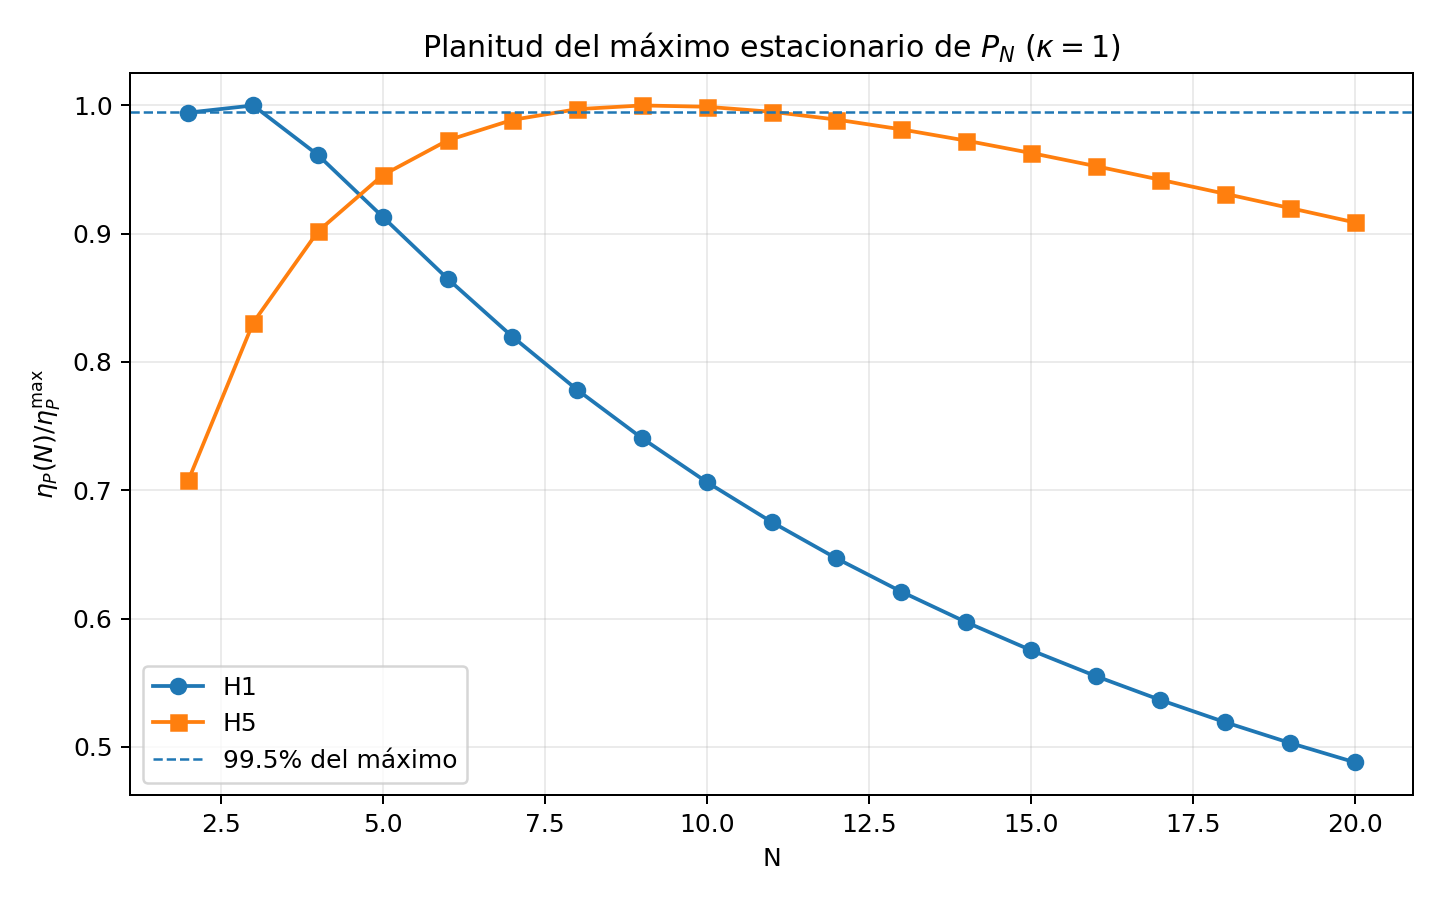
\includegraphics[width=0.84\textwidth]{figures/optimum_flatness.png}
\caption{Normalized stationary index of $P_N$ for $\kappa=1$. The dashed line represents $99.5\%$ of the maximum. In $H_1$, only $P_3$ belongs to that band; in $H_5$, the band contains $P_8,P_9,P_{10},P_{11}$.}
\label{fig:optimum-flatness}
\end{figure}

\begin{table}[htbp]
\centering
\scriptsize
\caption{Practical minimizers obtained by the complete sweep. The ``1 cycle'' column gives the first index of each family that meets the tolerance in the initial cycle; in that cycle $P_j$ and $S_j$ execute exactly the same block. Times are medians with IQR in parentheses, in milliseconds. Work corresponds to $\kappa=1$ and is used only as an algebraic reference.}
\label{tab:practical-minima-P-S}
\begin{tabular}{cccccccc}
\toprule
Field & $\delta$ & 1 cycle & best $P_N$ & wall time $P$ & best $S_m$ & wall time $S$ & work $P/S$\\
\midrule
$H_1$ & 0.10 & 5 & $P_5$ (1) & $0.1188\,(0.0047)$ & $S_5$ (1) & $0.1201\,(0.0041)$ & $12920/12920$\\
$H_1$ & 0.30 & 7 & $P_2$ (2) & $0.1429\,(0.0040)$ & $S_2$ (2) & $0.1360\,(0.0084)$ & $15160/14760$\\
$H_1$ & 0.60 & 9 & $P_2$ (2) & $0.1381\,(0.0119)$ & $S_2$ (2) & $0.1293\,(0.0040)$ & $15160/14760$\\
$H_5$ & 0.10 & 4 & $P_4$ (1) & $1.0738\,(0.1373)$ & $S_4$ (1) & $1.0549\,(0.1281)$ & $3541200/3541200$\\
$H_5$ & 0.30 & 5 & $P_5$ (1) & $0.9886\,(0.0410)$ & $S_5$ (1) & $0.9992\,(0.0678)$ & $3707400/3707400$\\
$H_5$ & 0.60 & 6 & $P_6$ (1) & $1.0562\,(0.1191)$ & $S_6$ (1) & $1.0743\,(0.1335)$ & $3873600/3873600$\\
\bottomrule
\end{tabular}
\end{table}

\begin{figure}[htbp]
\centering
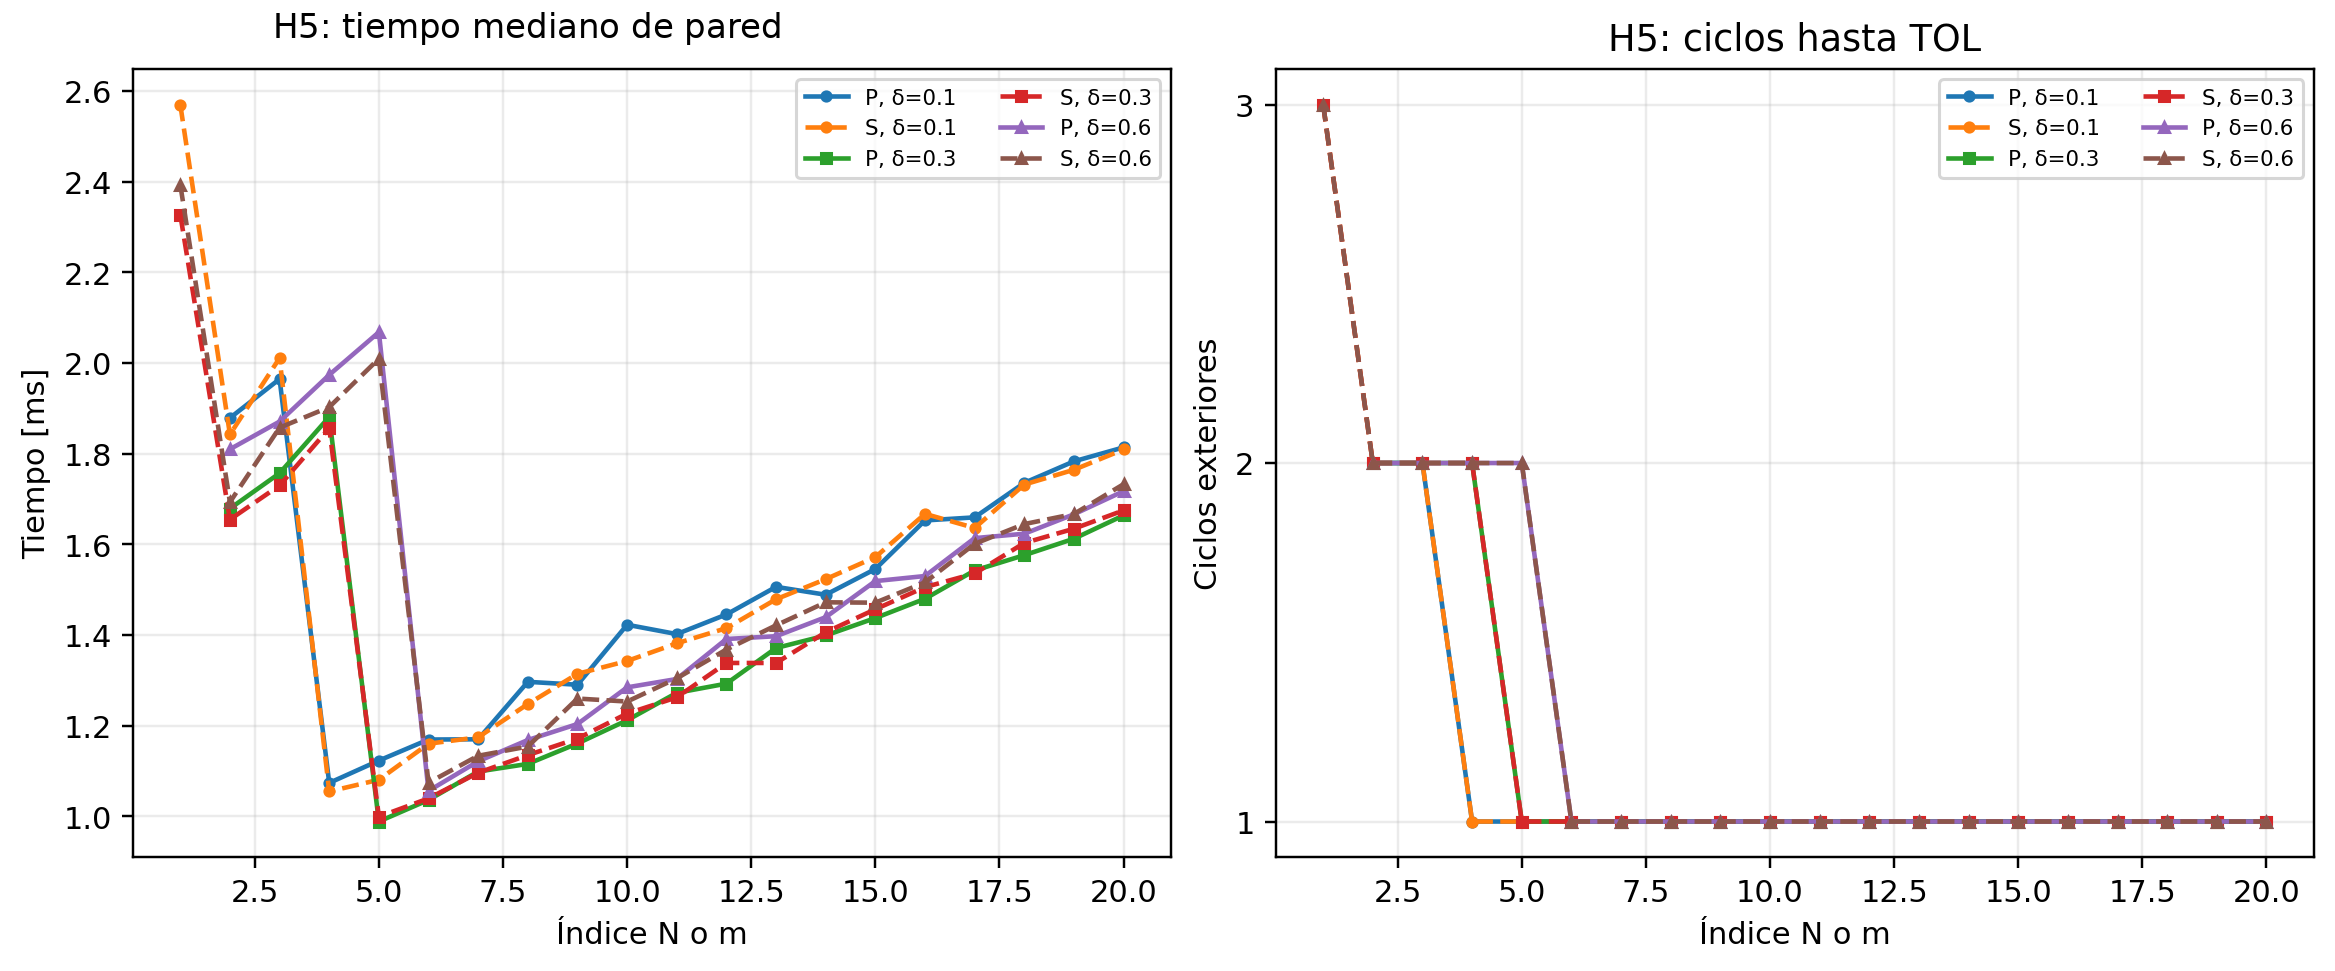
\includegraphics[width=0.96\textwidth]{figures/H5_time_cycles.png}
\caption{Complete sweep in $H_5$ for three initial distances. Left: median elapsed wall time. Right: number of outer cycles required to reach $\mathrm{TOL}=10^{-12}$. The first cycle of $P_N$ and $S_N$ has the same resources. With more than one cycle, memory is active, but that activation does not imply a resolved timing separation; the curves are interpreted together with the IQRs in this supplement.}
\label{fig:H5-practical-sweep}
\end{figure}

\FloatBarrier

\subsection{Fusion resource counts and complete-solve summaries}
\begin{table}[htbp]
\centering
\scriptsize
\caption{Exact resource counts for the fused comparison. Values
in parentheses correspond to $N=2$. The ``end-to-end'' row
includes the common terminal evaluation of $F$ used by the stopping criterion.}
\label{tab:fusion-resource-accounting}
\begin{tabularx}{\textwidth}{Xlccccc}
\toprule
Regime & Method & $F$ & $J$ & LU & Solves & Matrix--vector products\\
\midrule
Stationary
& $\widehat P_N$
& $2N\;(4)$ & $2$ & $1$ & $(N+1)(N+3)\;(15)$ & $(N+1)^2\;(9)$\\
& $P_N\circ P_N$
& $2N\;(4)$ & $2$ & $2$ & $2(N+1)\;(6)$ & $0$\\
\addlinespace
First D macrocycle, before the residual
& $\widehat P_N$
& $2N\;(4)$ & $2$ & $1$ & $N^2+3N+1\;(11)$ & $N(N+1)\;(6)$\\
& $P_N\circ P_N$
& $2N\;(4)$ & $2$ & $2$ & $2N+1\;(5)$ & $0$\\
\addlinespace
End-to-end, one macrocycle, with terminal residual
& $\widehat P_N$
& $2N+1\;(5)$ & $2$ & $1$ & $N^2+3N+1\;(11)$ & $N(N+1)\;(6)$\\
& $P_N\circ P_N$
& $2N+1\;(5)$ & $2$ & $2$ & $2N+1\;(5)$ & $0$\\
\bottomrule
\end{tabularx}
\end{table}

\begin{table}[htbp]
\centering
\small
\caption{Practical end-to-end comparison of $\widehat P_2$ versus $P_2\circ P_2$. Work includes the common terminal evaluation of $F$ listed in \cref{tab:fusion-resource-accounting}. Negative values favor fusion.}
\label{tab:fusion-practical}
\begin{tabular}{crrrc}
\toprule
$n$ & Median $\Delta W$ [\%] & Median $\Delta t$ [\%] & Range $\Delta t$ [\%] & clear differences/$18$\\
\midrule
40  & $-2.5$  & $+30.9$ & $[+23.2,+35.2]$ & $4/18$\\
55  & $-10.1$ & $+24.1$ & $[+18.3,+26.5]$ & $7/18$\\
100 & $-23.3$ & $+12.2$ & $[+8.7,+15.0]$  & $0/18$\\
200 & $-34.6$ & $-29.4$ & $[-30.9,-27.6]$ & $16/18$\\
\bottomrule
\end{tabular}
\end{table}

\begin{table}[htbp]
\centering
\small
\caption{Secondary nearby-order comparison of $\widehat P_2$ and $P_{10}$. Define
$\Delta W=100(W_{\widehat P_2}/W_{P_{10}}-1)$ and
$\Delta t=100(t_{\widehat P_2}/t_{P_{10}}-1)$; negative values favor $\widehat P_2$. The timing columns summarize the nine combinations of $\delta$ and tolerance per field.}
\label{tab:Phat2-P10}
\begin{tabular}{crrrrrc}
\toprule
Field & $n$ & $10^6\eta_{\widehat P_2}/10^6\eta_{P_{10}}$ &
$\Delta W$ [\%] & median $\Delta t$ [\%] & range $\Delta t$ [\%] & clear/$9$\\
\midrule
$H_3$ & 100 & $3.32012/3.17369$ & $-12.35$ & $+1.31$ & $[-2.20,+3.62]$ & $0/9$\\
$H_5$ & 200 & $0.571324/0.554943$ & $-8.67$ & $-0.76$ & $[-4.07,+1.41]$ & $0/9$\\
\bottomrule
\end{tabular}
\end{table}

\FloatBarrier

\clearpage
\subsection{Consecutive truncation parameters}
\begin{table}[ht]
\centering
\caption{Measured COC for $q=N+1$ and $q=N+2$ in the coupled polynomial stress field used for order verification.}\label{tab:q-coc}
\begin{tabular}{cccc}
\toprule
$N$&$q$&reference order&observed COC\\
\midrule
2&3&10.89897949&10.87757519\\
2&4&11.65685425&11.67053004\\
3&4&19.16515139&19.15817198\\
3&5&20.80776406&20.81728526\\
4&5&29.31782106&29.31487833\\
4&6&31.87450787&31.88067604\\
\bottomrule
\end{tabular}
\end{table}

\FloatBarrier

\end{document}
